\chapter{Observations and findings}
This chapter consists of results of Python code that implemented genetic algorithm. The code can be found at a dedicated github repository \citep{github} created for this thesis. Here's the link for the repository:

\url{https://github.com/iamstarstuff/MScDataScienceThesis}

The `EDA.ipynb' Jupyter notebook file has the exploratory data analysis code and `Final Compiled.ipynb' notebook has the machine learning models and genetic algorithm implementation.

The data downloaded from the SDSS SQL query server file name `Skyserver\_SQL5\_24\_2023 12\_41\_33 PM.csv' is also available on the repository.

\section{EDA}

Initial exploratory data analysis (EDA) was performed to gain deeper insights into the dataset. The dataset is of the shape (500000,18) i.e., 500 thousand rows and 18 columns. Of these 18 columns most of the columns are essentially metadata associated with each object. There are three unique classes of objects in our dataset which can be seen from \textit{`class'} column. It is important to know the count of each class to determine if our dataset is balanced or imbalanced. \autoref{fig:classdistribution} shows that the dataset is balanced with more than half the objects belonging to the class 'GALAXY', about 39\% of the objects belong to the class `STAR' and 11\% belong to the class `QSO'. QSO stands for Quasi-Stellar objects, also known as Quasars. This shows clear imbalance of classes and this should be taken into account during training in order to ensure that our machine learning model takes it into consideration and learns all classes proportionally. This can be done using the StratifiedKFold cross validation technique, refer \autoref{fig:cv}.

\autoref{fig:3dmap} shows the distribution of class of astronomical objects in the sky. Interestingly there are cluster of observations when only stars were observed. One other peculiar thing we can observe is how the observations are distributed in 2 seperated hemishpheres. The SDSS telescope, like many other ground-based telescopes, has limitations when it comes to observing objects at the zenith, which is the point directly overhead in the sky. This limitation is primarily due to the design and mechanics of the telescope, as well as the Earth's atmosphere. Telescopes are complex instruments with mechanical systems for pointing and tracking celestial objects. Some telescopes may have limitations in their mechanical range of motion, preventing them from pointing directly overhead.

\begin{table}[H]
\begin{center}
\caption{SDSS DR18 Columns and Description.}
\label{tab:column_description}
\begin{tabular}{|c|p{10cm}|}
\hline
\textbf{Column Name} & \textbf{Description} \\
\hline
objid & The unique identifier for the object in the PhotoObj table. \\
\hline
ra & The right ascension of the object in degrees. \\
\hline
dec & The declination of the object in degrees. \\
\hline
u, g, r, i, z & The magnitudes of the object in different bands (ultraviolet, green, red, near-infrared, and infrared). \\
\hline
run & The specific run in which the object was observed. \\
\hline
rerun & The rerun number for the run. \\
\hline
camcol & The camera column number. \\
\hline
field & The field number. \\
\hline
specobjid & The unique identifier for the object in the SpecObj table. \\
\hline
class & The classification of the object (e.g., star, galaxy, quasar). \\
\hline
z as redshift & The redshift value of the object, indicating its recession velocity. \\
\hline
plate & The plate number on which the object was observed. \\
\hline
mjd & The Modified Julian Date (MJD) of the observation. \\
\hline
fiberid & The fiber identification number. \\
\hline
\end{tabular}
\end{center}
\end{table}

The data required no cleaning as it has no null values or infinities that could cause problems with training. There were no missing values as well in the dataset which was verified with the pandas functions for these operations. Correlation matrix is a great way to identify potential features, so only those columns with higher correlation than other columns were selected. 
\begin{figure}
    \centering
    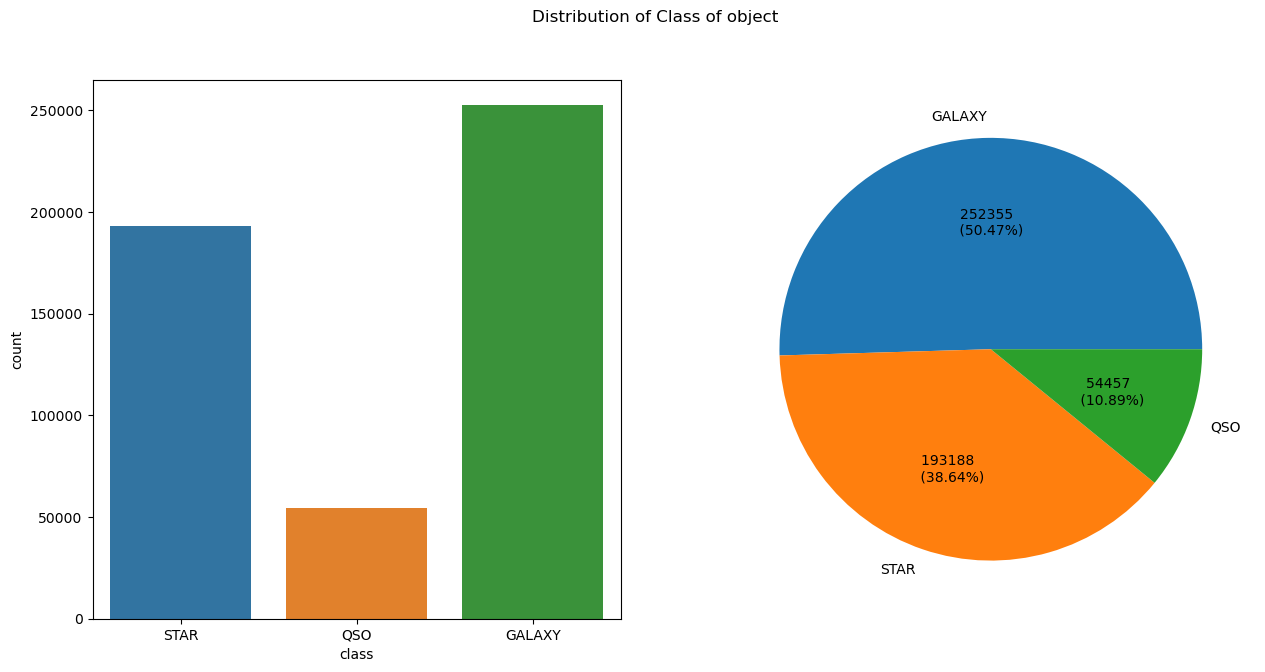
\includegraphics[scale=0.5]{images/Distribution of class.png}
    \caption{Distribution of Class of objects}
    \label{fig:classdistribution}
\end{figure}


\begin{figure}
    \centering
    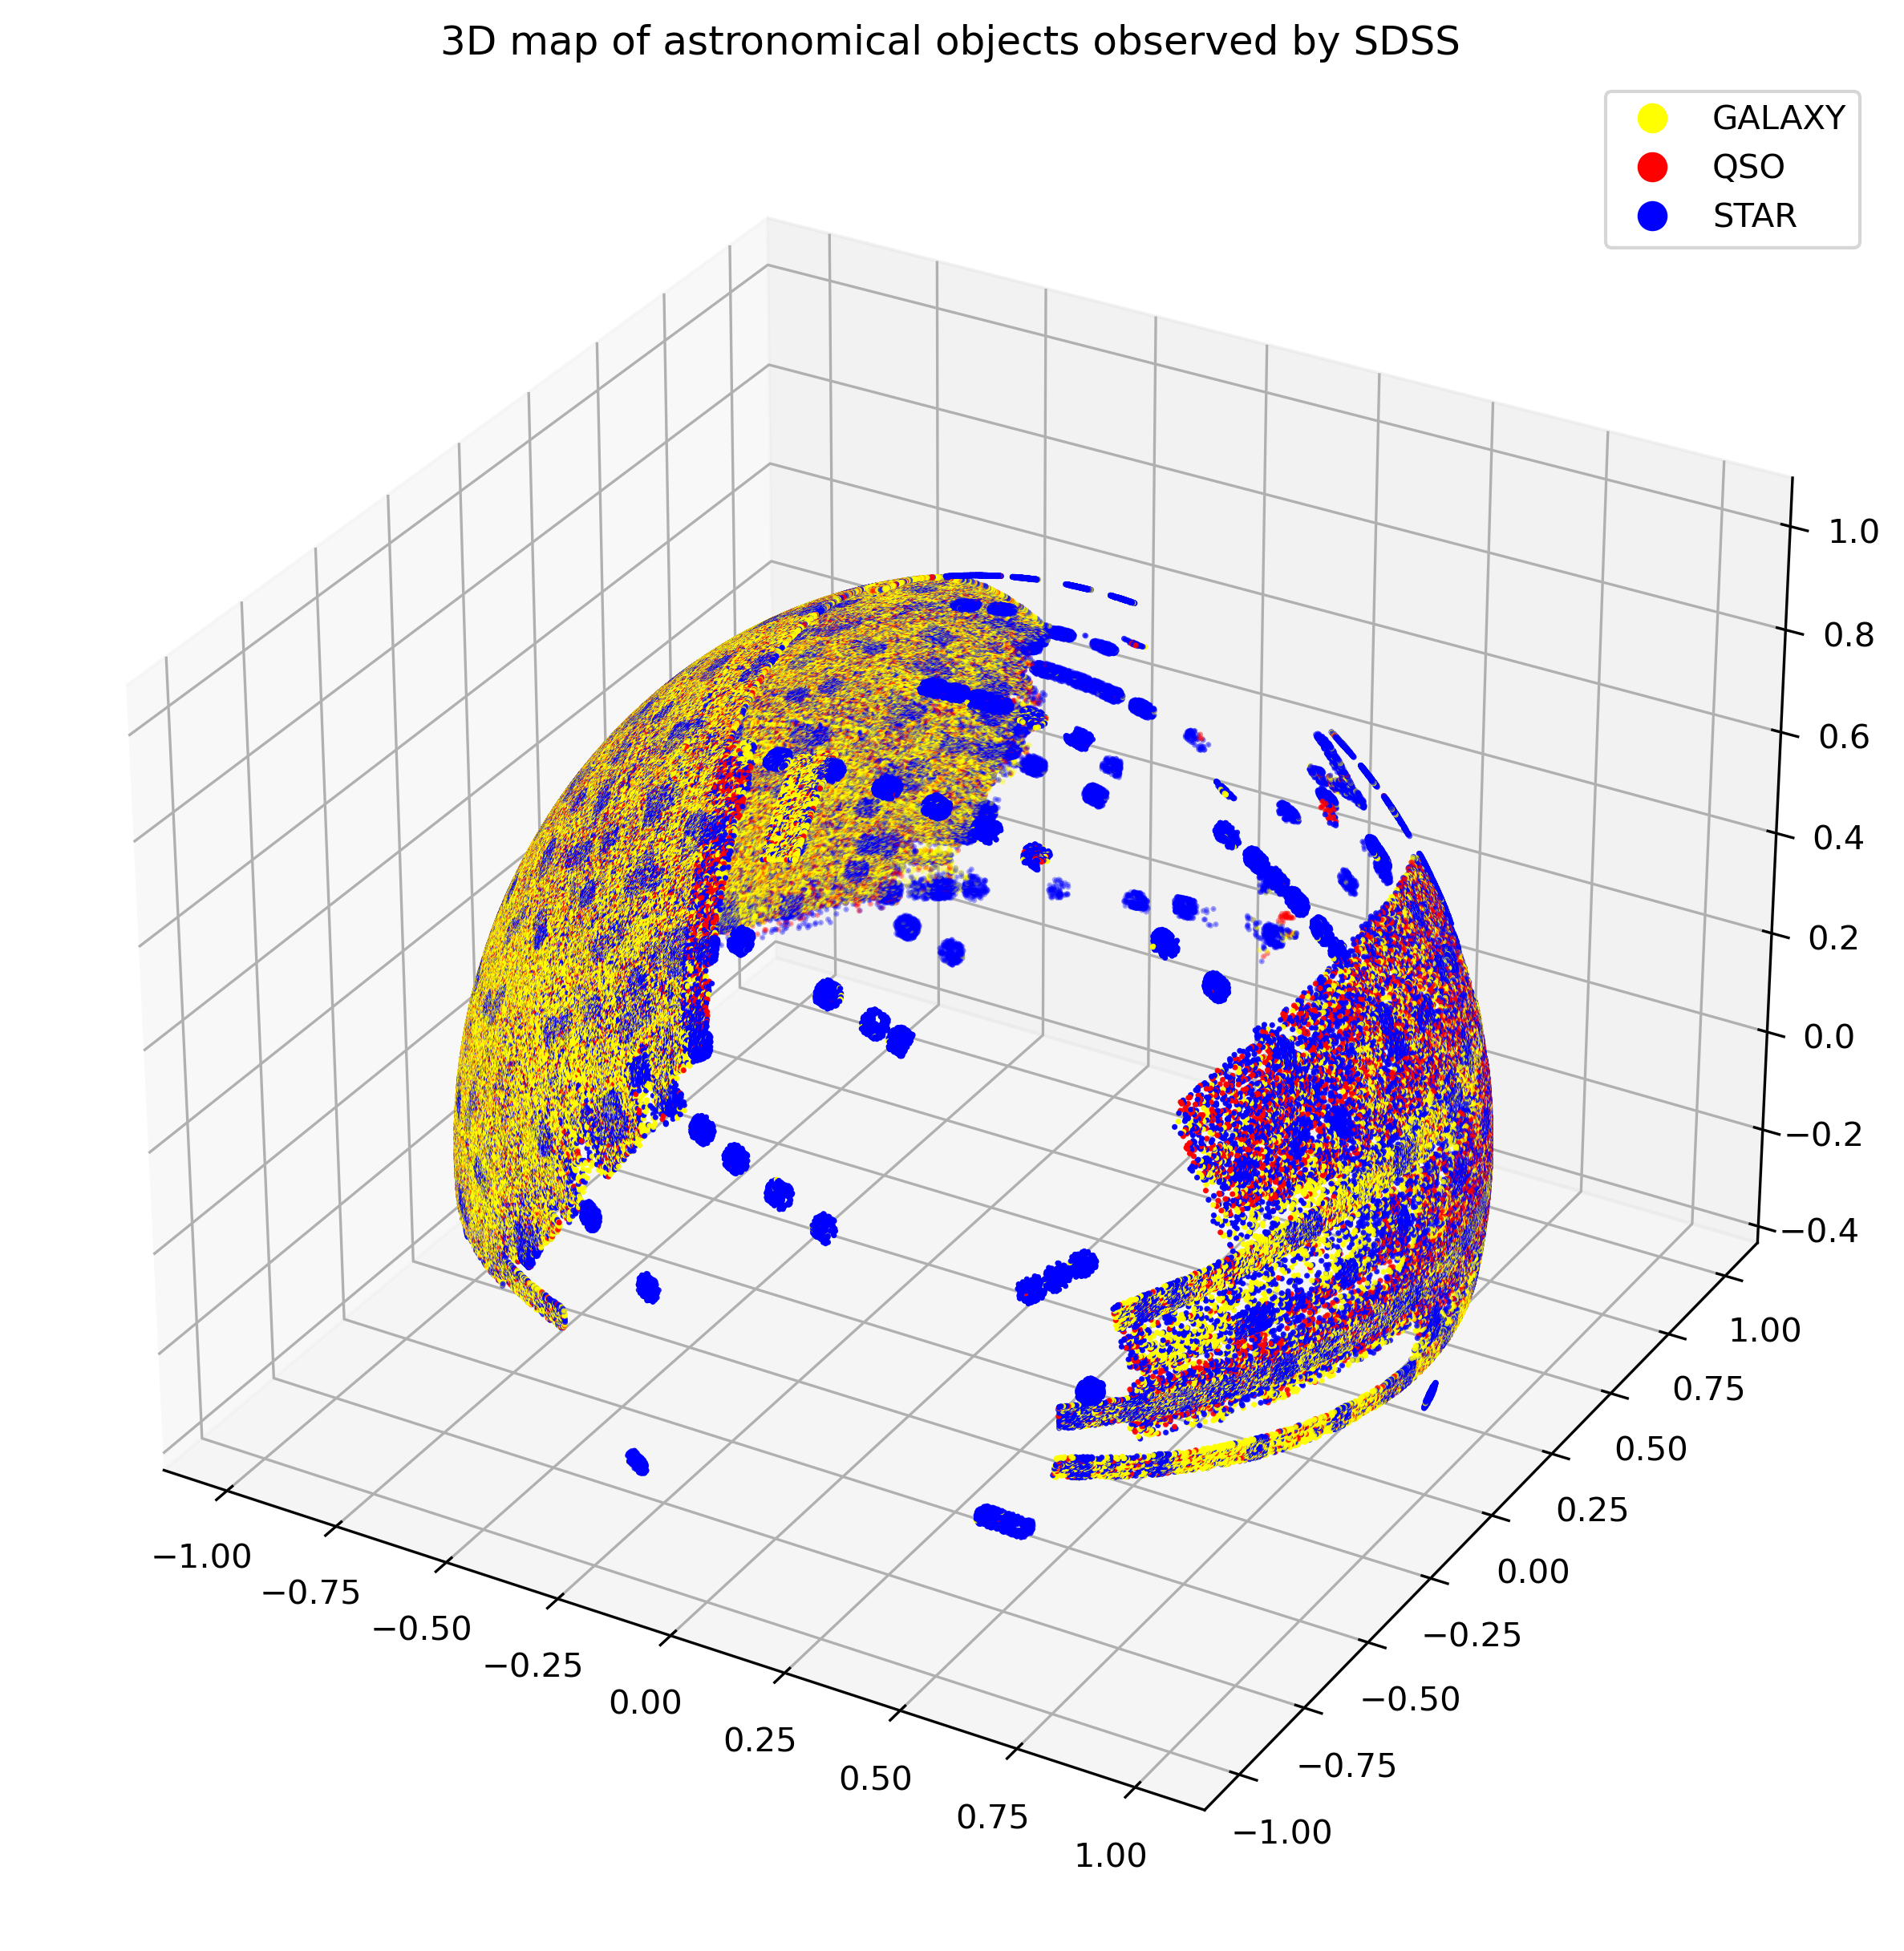
\includegraphics[scale=0.7]{images/3dmap.png}
    \caption{3D Map of astronomical objects based on coordinates}
    \label{fig:3dmap}
\end{figure}



Of these columns the correlation between class of object is highest with columns like the color bands $u$, $g$, $r$, $i$, $z$ and redshift. Due to this only these columns were selected as features for training. 

\begin{figure}[H]
    \centering
    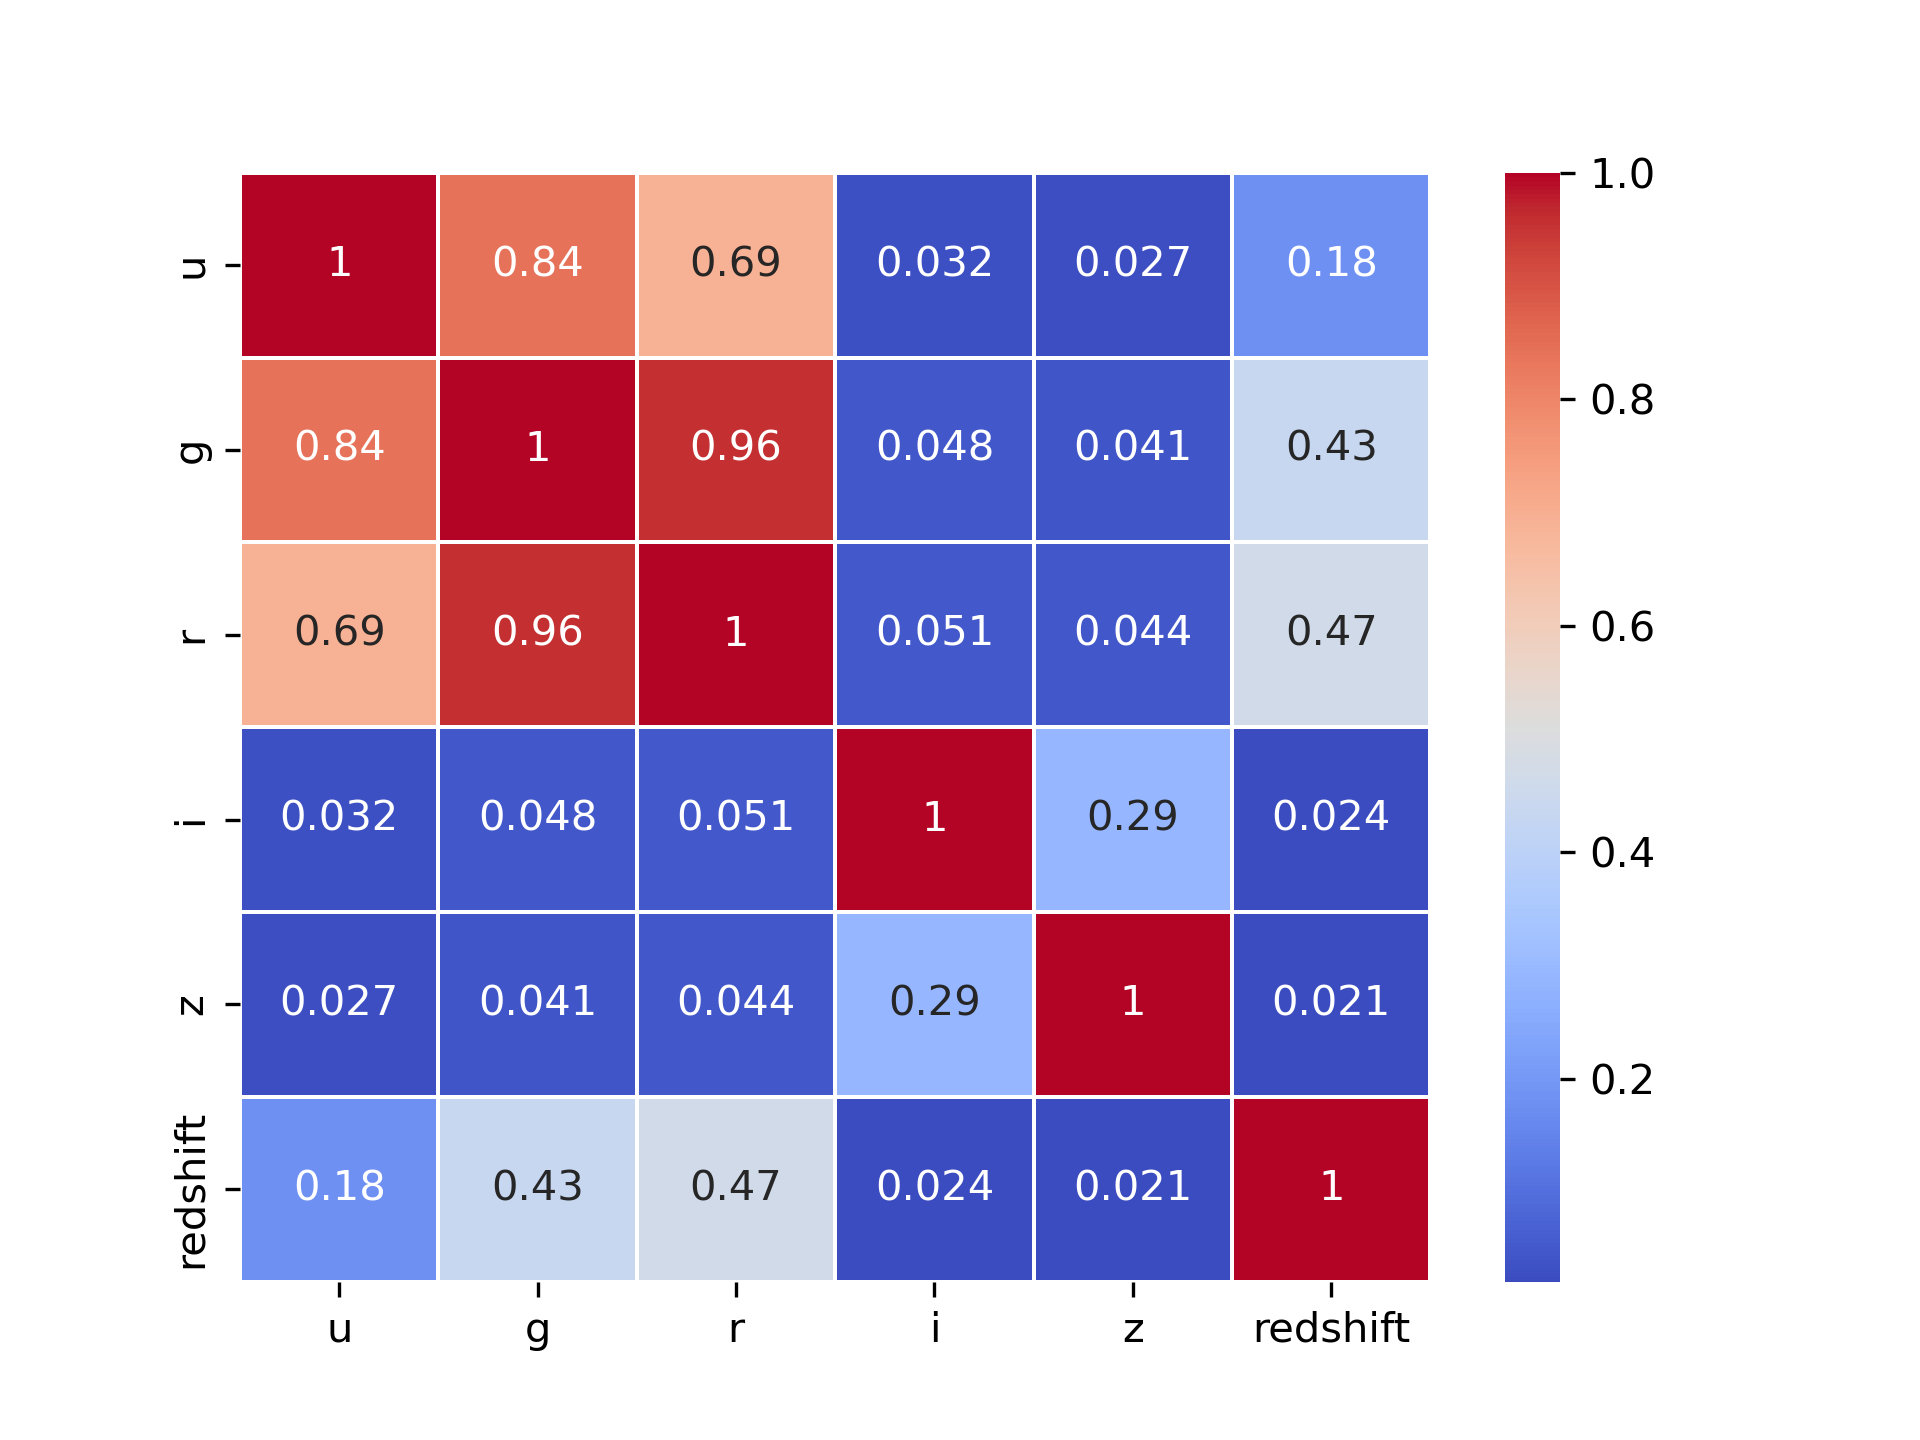
\includegraphics[scale=1]{images/CorrelationMatrix.png}
    \caption{Correlation matrix of the color filters and redshift.}
    \label{fig:corr}
\end{figure}


% \begin{landscape}
%     \begin{figure}[ht]
%         \begin{minipage}[b]{0.5\linewidth}
%             \centering
%             \begin{subfigure}{\textwidth}
%                 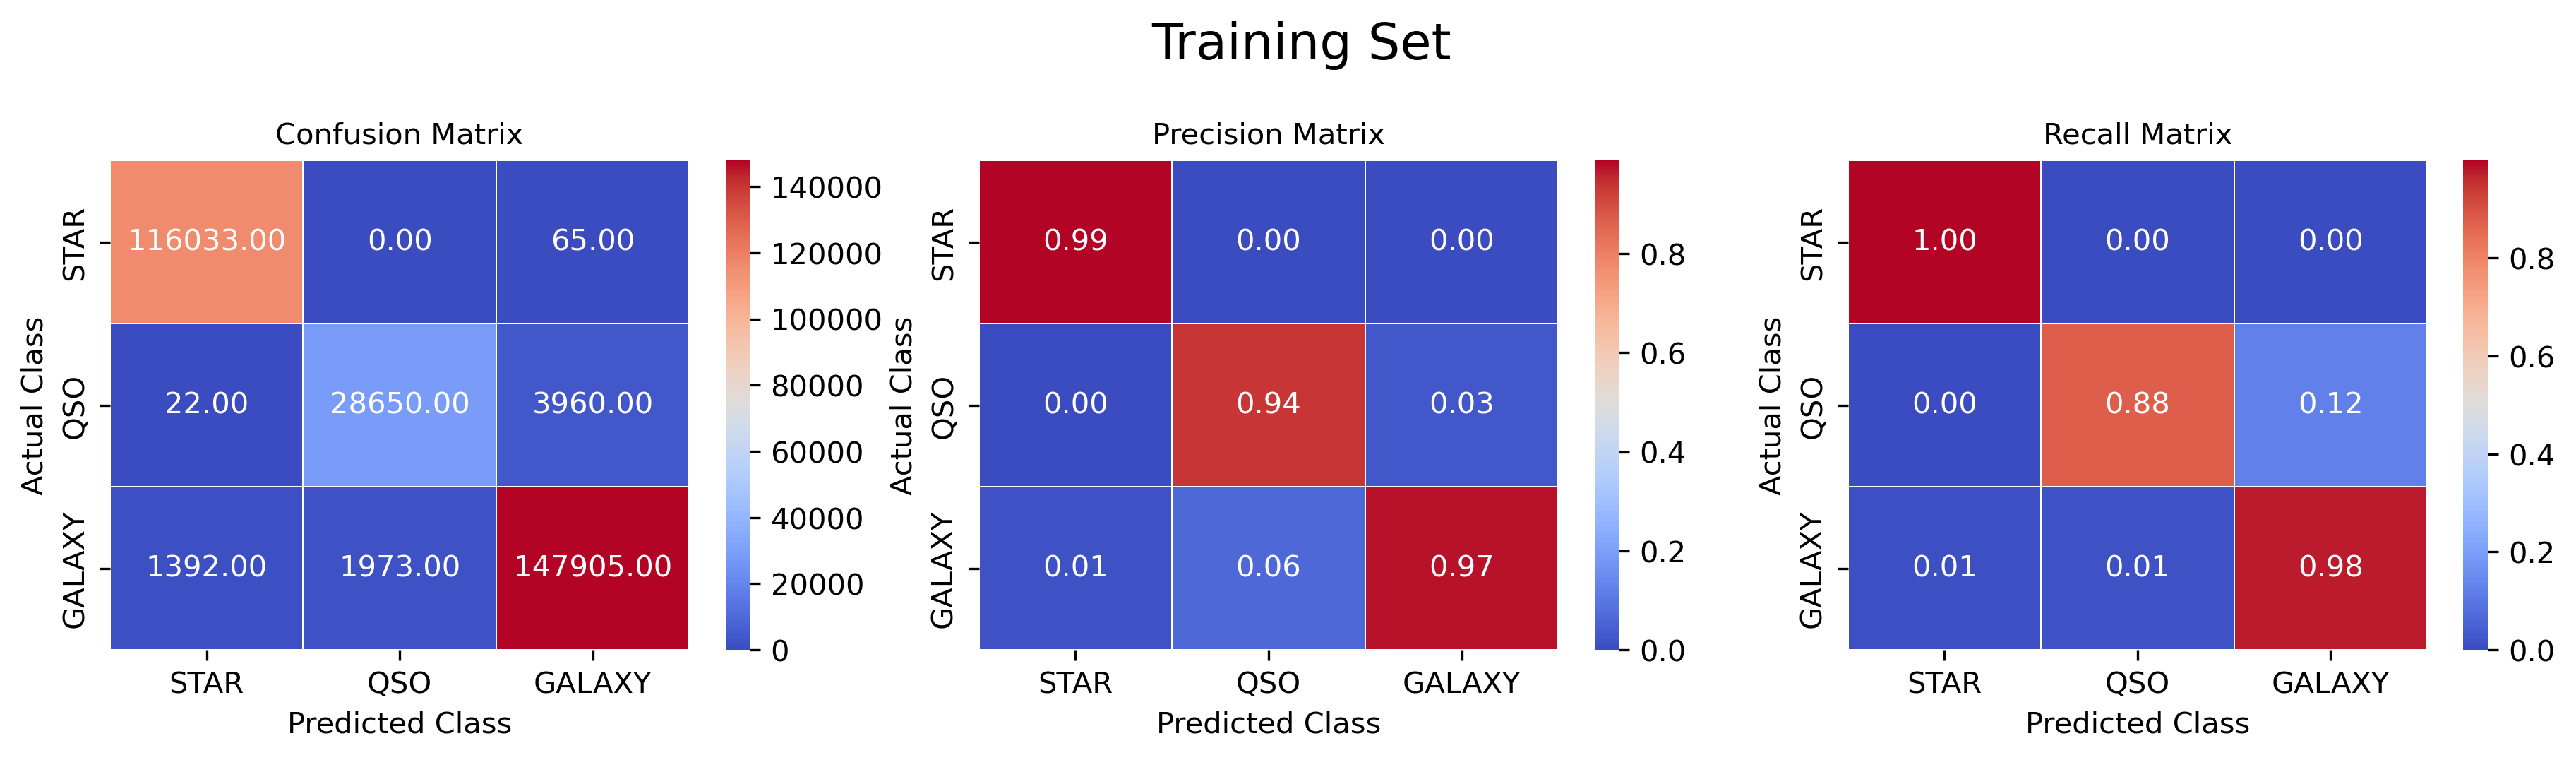
\includegraphics[width=\linewidth]{images/Baseline_RFC_Train.png}
%                 \caption{(a) Training Set Confusion Matrix, Precision and Recall}
%                 \label{fig:BaselineRFCTrain}
%             \end{subfigure}
%             \begin{subfigure}{\textwidth}
%                 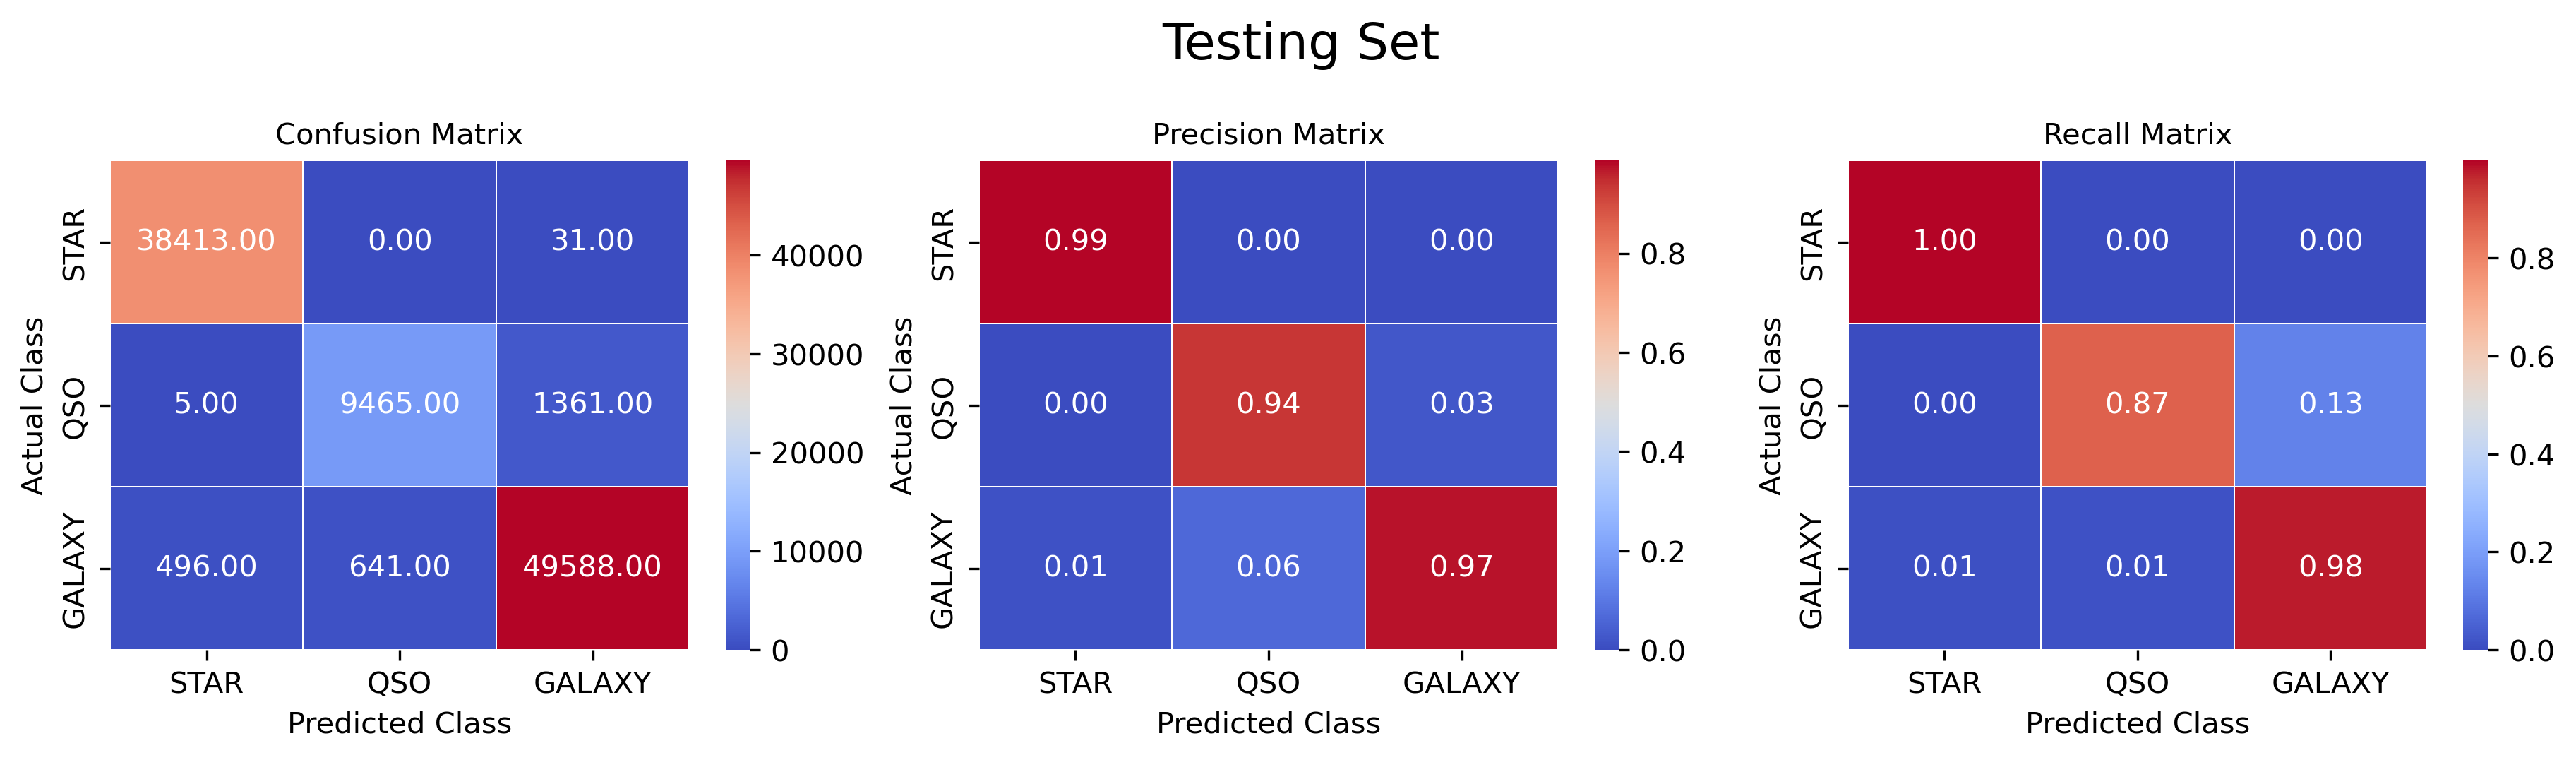
\includegraphics[width=\linewidth]{images/Baseline_RFC_Test.png}
%                 \caption{(a) Testing Set Confusion Matrix, Precision and Recall}
%                 \label{fig:BaselineRFCTest}
%             \end{subfigure}
%             \begin{subfigure}{\textwidth}
%                 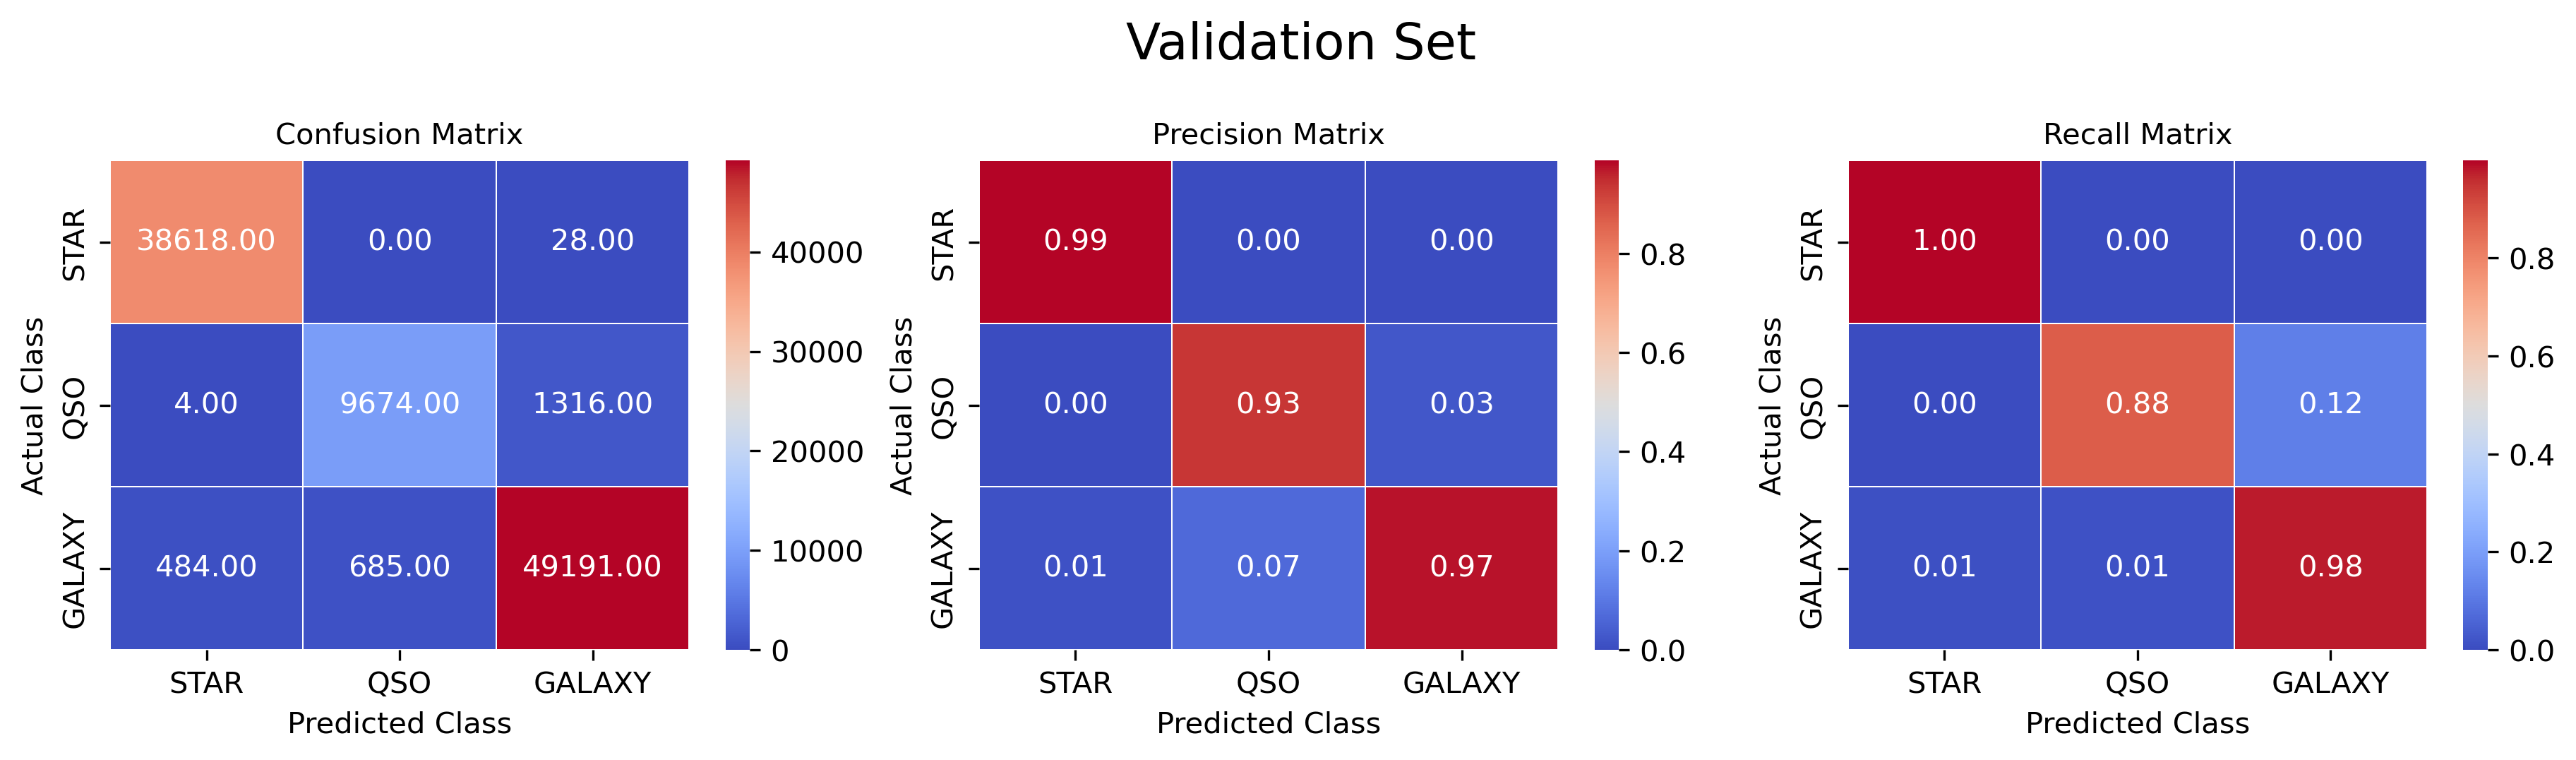
\includegraphics[width=\linewidth]{images/Baseline_RFC_Val.png}
%                 \caption{(a) Validation Set Confusion Matrix, Precision and Recall}
%                 \label{fig:BaselineRFCVal}
%             \end{subfigure}
%             \caption{Baseline performance of Random Forest Classifier}
%             \label{fig:BaselineRFC}
%         \end{minipage}
%         \begin{minipage}[b]{0.5\linewidth}
%             \centering
%             \begin{subfigure}{\textwidth}
%                 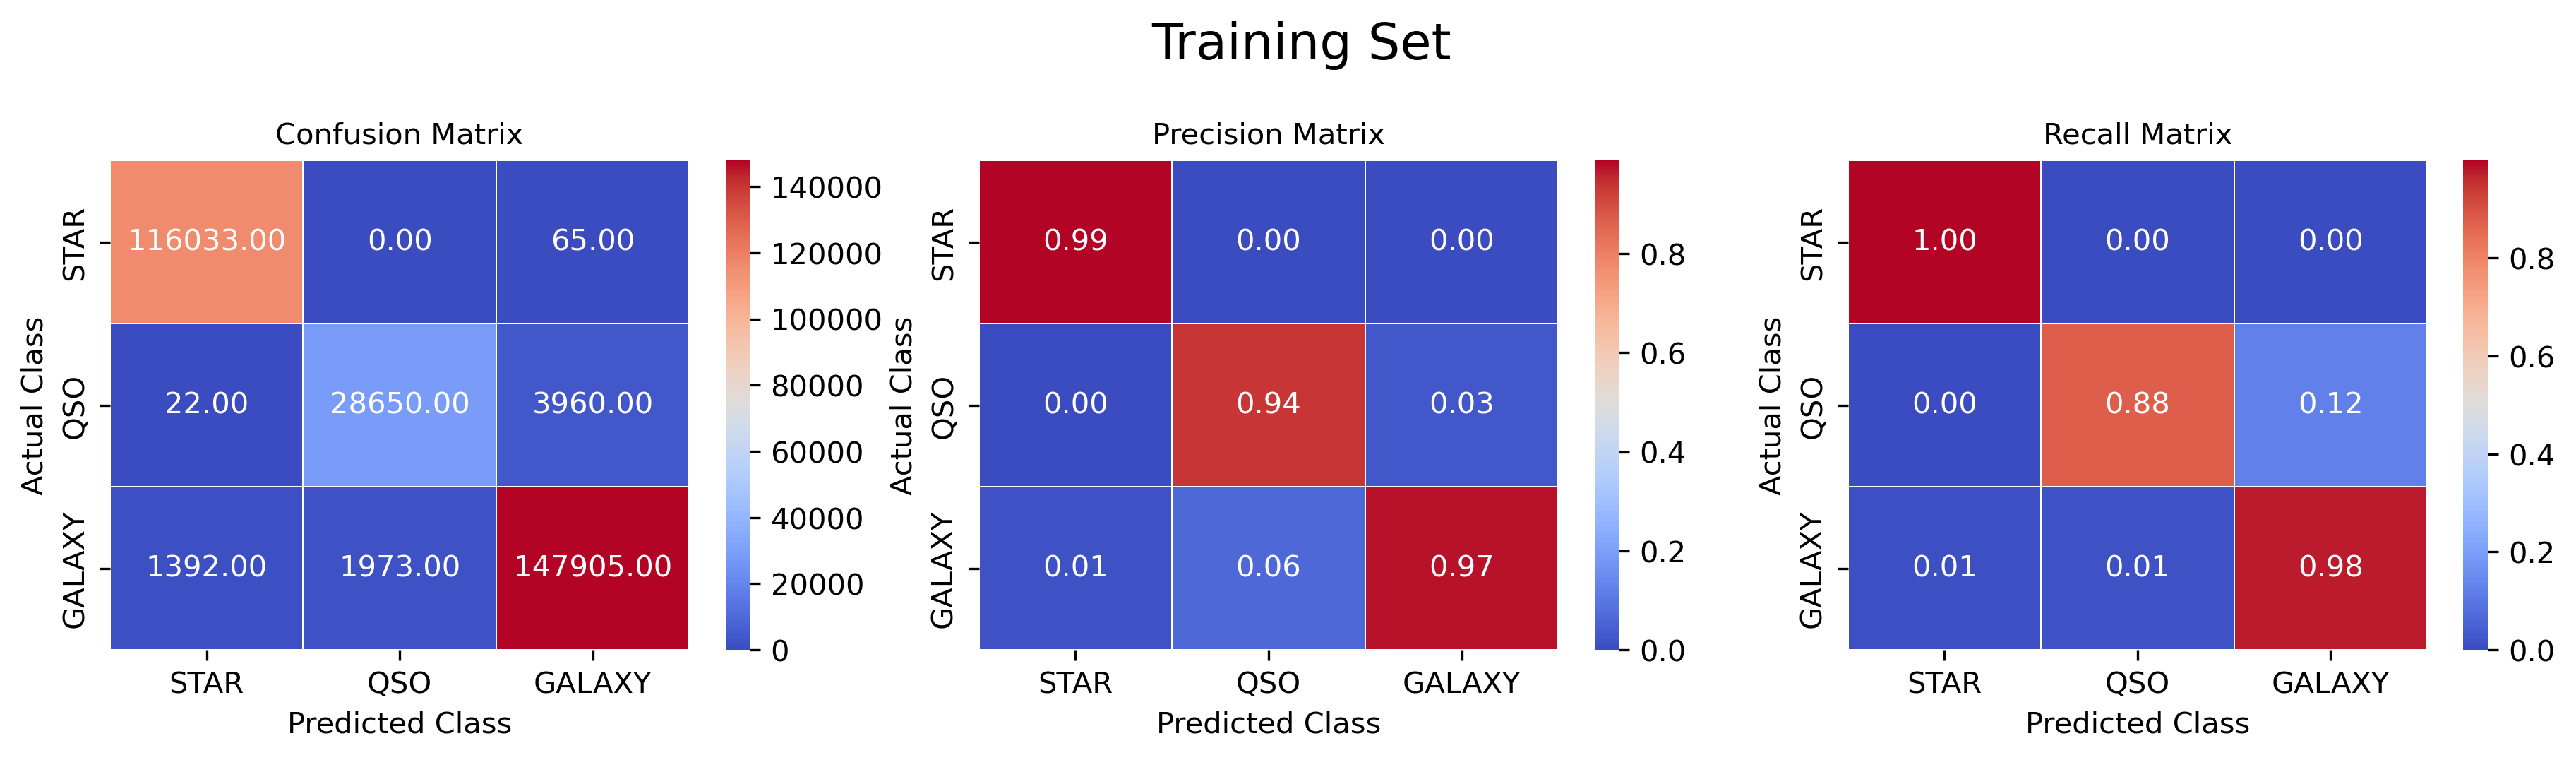
\includegraphics[width=\linewidth]{images/GA_RFC_Train.png}
%                 \caption{(a) Training Set Confusion Matrix, Precision and Recall}
%                 \label{fig:GARFCTrain}
%             \end{subfigure}
%             \begin{subfigure}{\textwidth}
%                 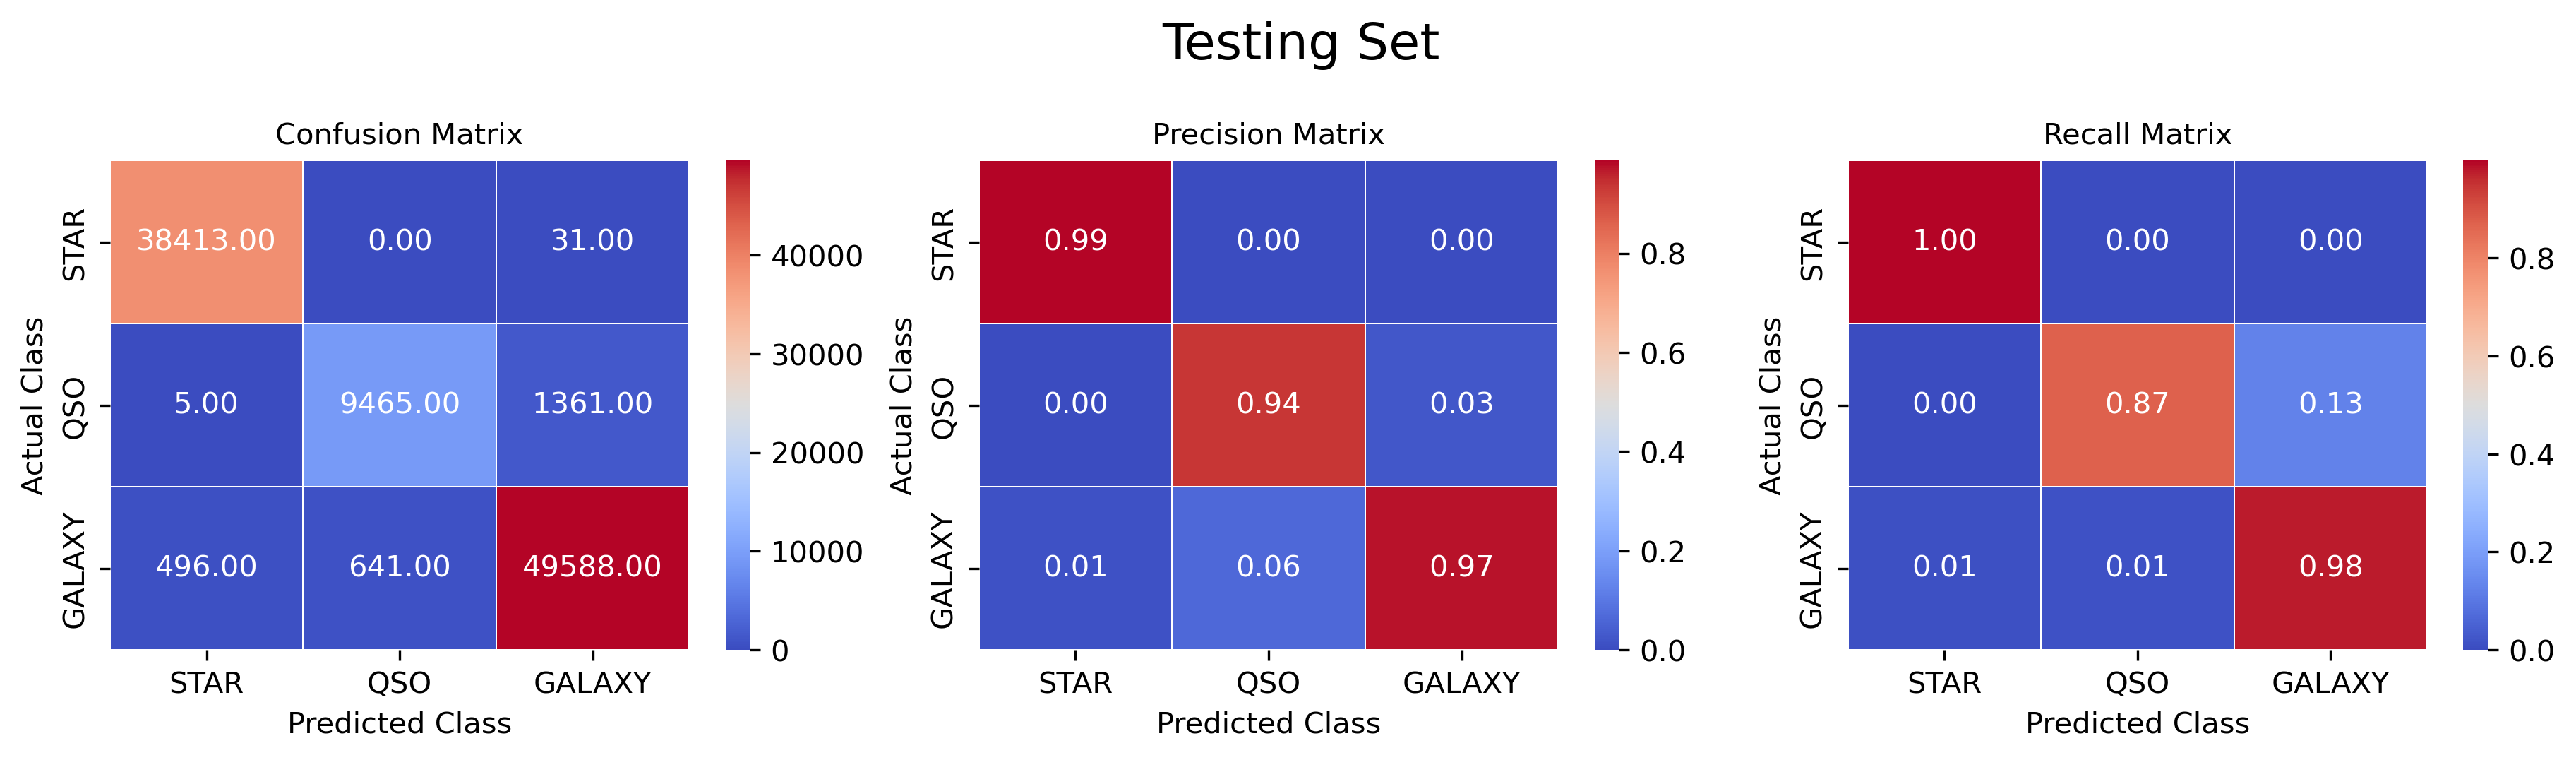
\includegraphics[width=\linewidth]{images/GA_RFC_Test.png}
%                 \caption{(a) Testing Set Confusion Matrix, Precision and Recall}
%                 \label{fig:GARFCTest}
%             \end{subfigure}
%             \begin{subfigure}{\textwidth}
%                 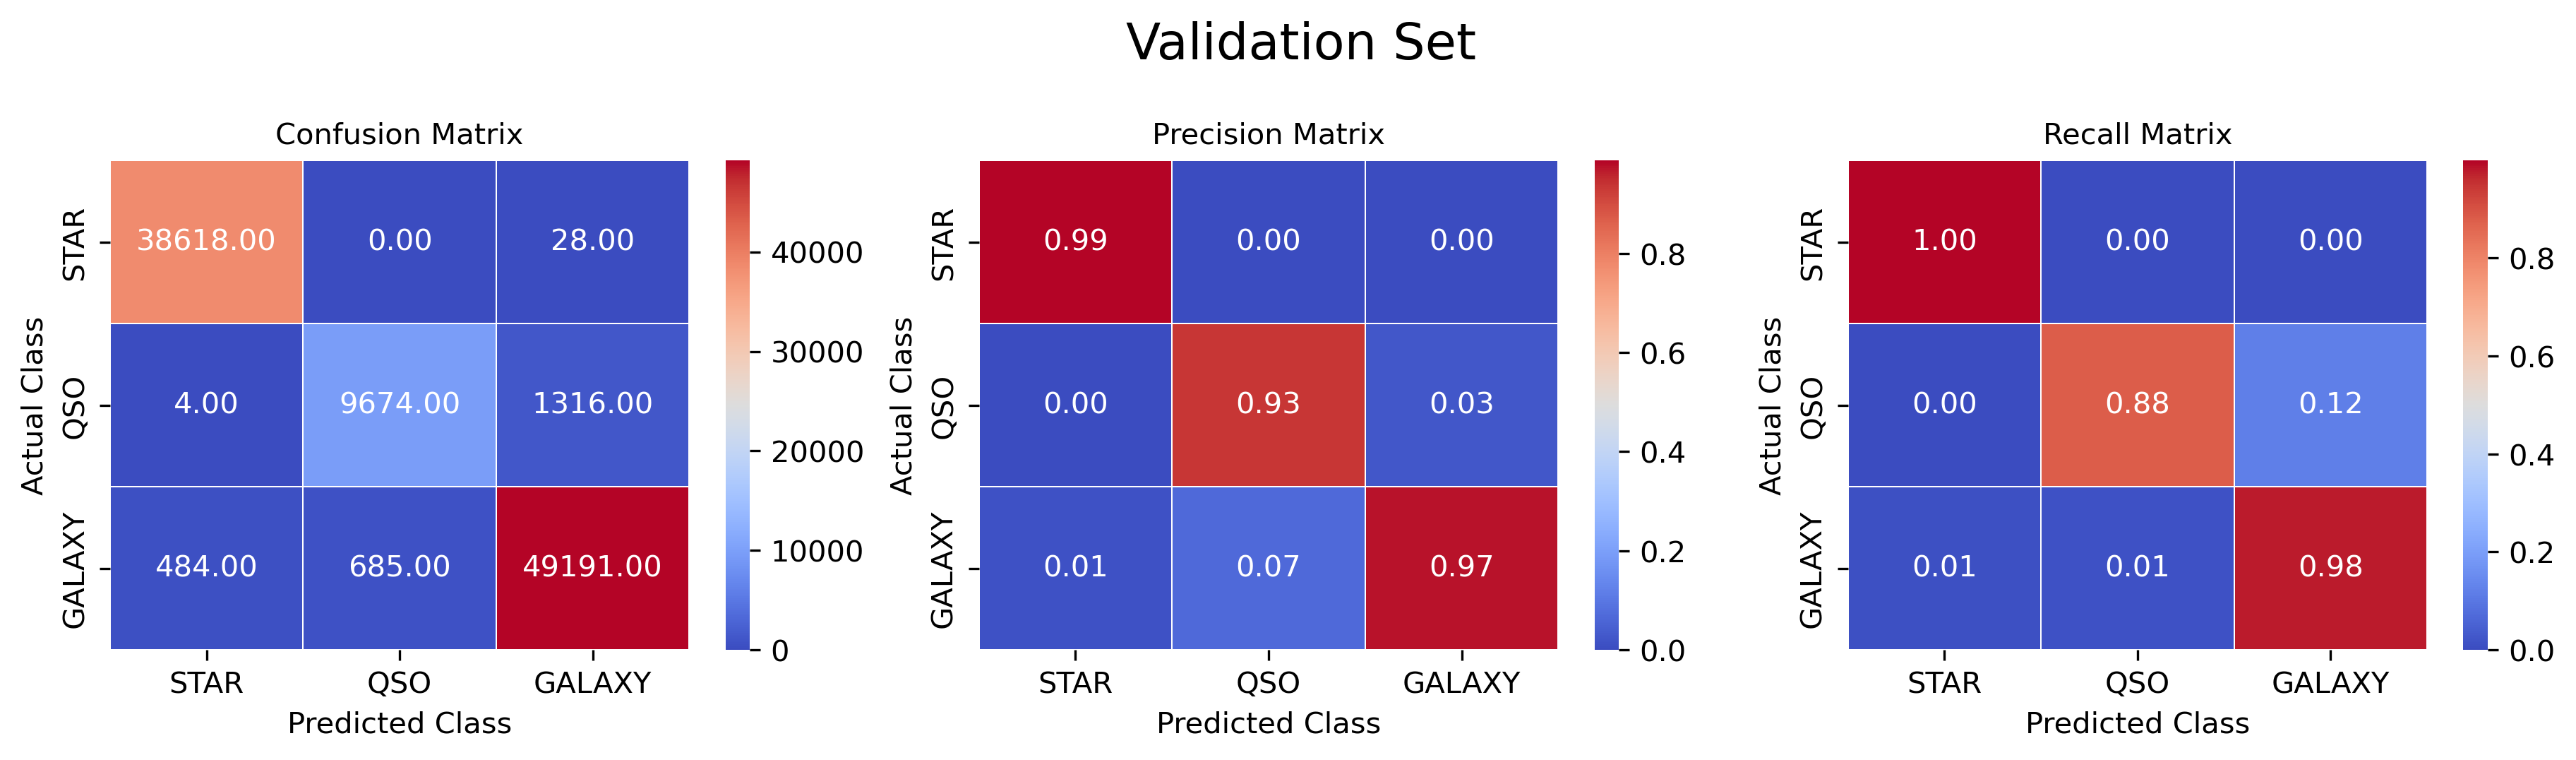
\includegraphics[width=\linewidth]{images/GA_RFC_Val.png}
%                 \caption{(a) Validation Set Confusion Matrix, Precision and Recall}
%                 \label{fig:GARFCVal}
%             \end{subfigure}
%             \caption{Performance of Random Forest Classifier after Genetic optimisation}
%             \label{fig:GARFC}
%         \end{minipage}
%     \end{figure}
% \end{landscape}
In the same way that I wrote a custom function to split data, I wrote a custom function to display evaluation metrics for the models. These function were heavily inspired from work done by \cite{towardsdatascienceStellarClassification}. The function plots confusion matrix for precision scores and recall scores, prints classification report and also prints logloss values. This enables quick report of model performance with all the necessary metrics required.

\section{Model Performance}
In this section, we will go through performance metrics of the models and also compare the performance after genetic optimisation.

\subsection{Random Forest Classifier}

To establish baseline performance of Random Forest classifier, the model was first trained using the default hyperparamters. 

\begin{lstlisting}[language=Python]
    rfc = RandomForestClassifier(random_state=random_seed)
    rfc.fit(X_train,y_train)
\end{lstlisting}

After training the model with default hyperparameters, accuracy score of 0.97 was obtained both on testing and validation datasets. \autoref{fig:BaselineRFC} shows the training, testing and validation confusion matrices with precision and recall scores. From the figure, we can see that the model is able to capture the patterns and accurately predict the class of object. Even the validation dataset has a good average recall of 0.95. However, due to such high scores one can suspect that overfitting might be taking place. To address this we can look at other evaulation metrics like  precision and f1 score to determine if overfitting is the case or not.

\begin{figure}[H] 
    \centering
    \begin{subfigure}{\textwidth}
        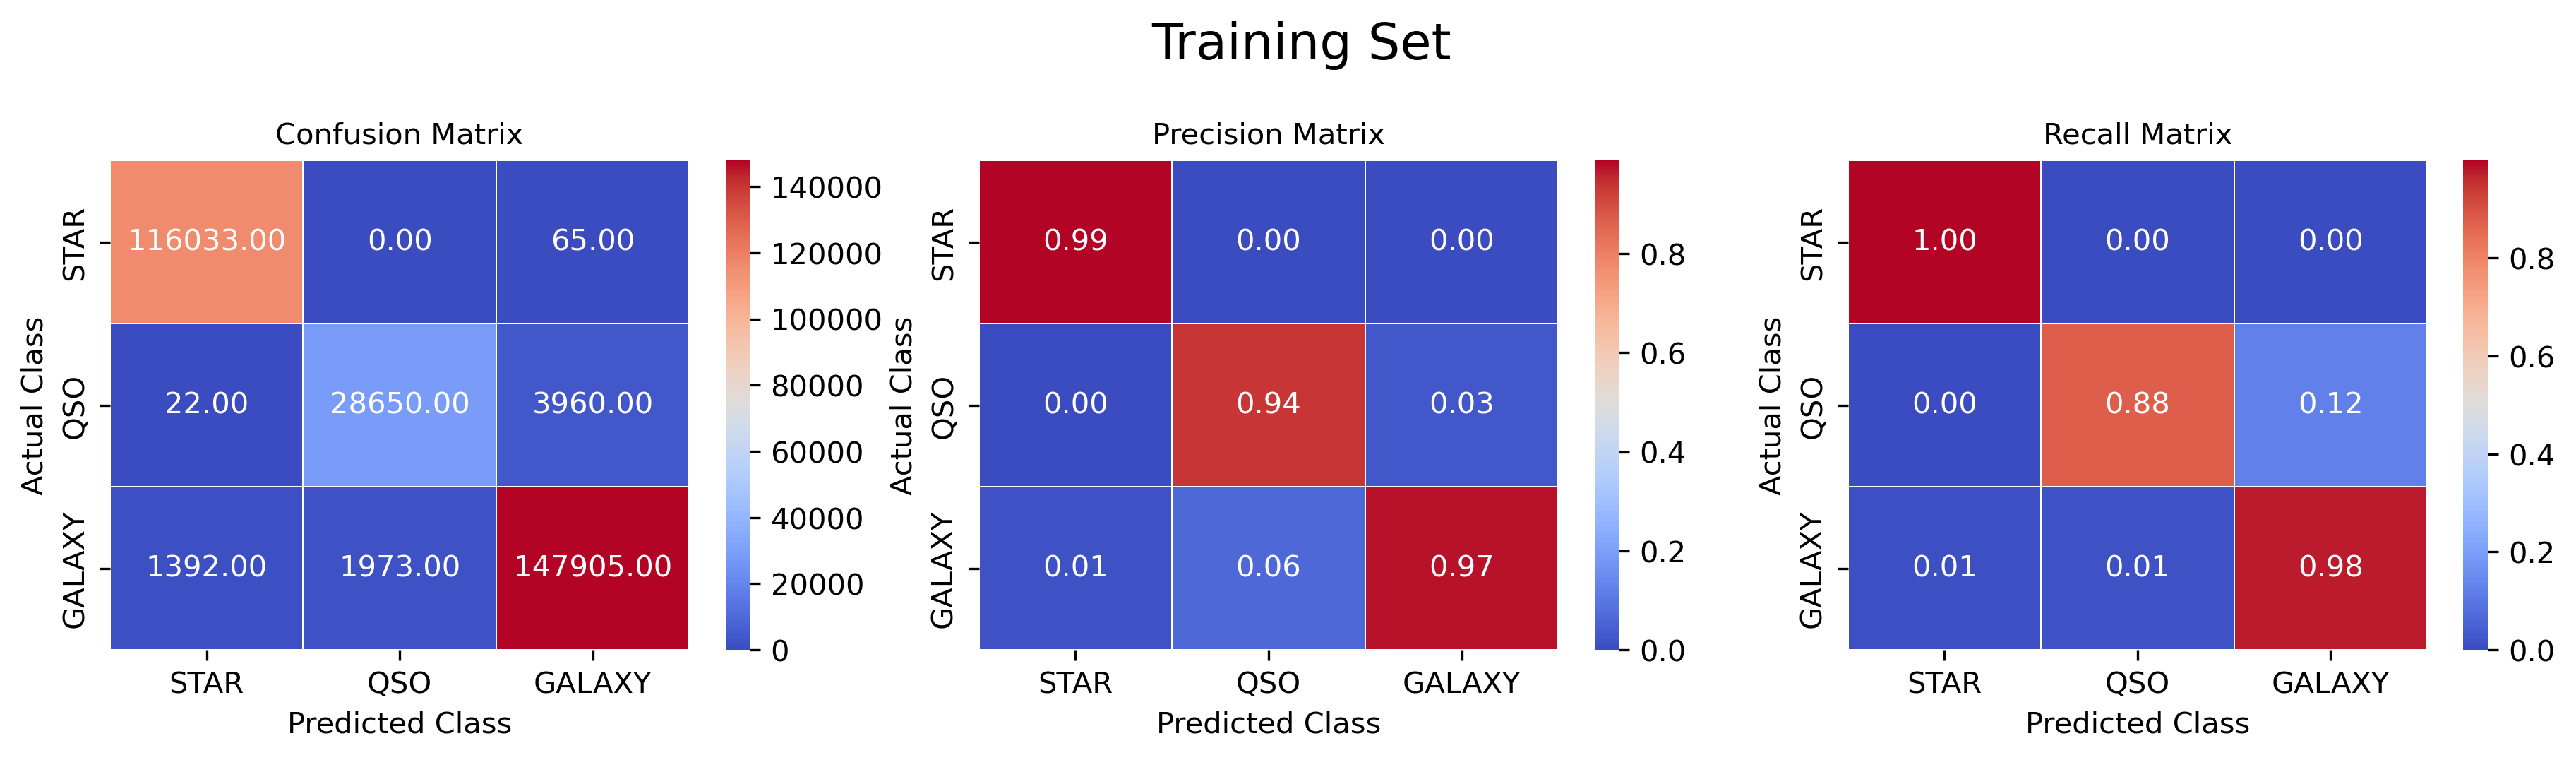
\includegraphics[width=\linewidth]{images/Baseline_RFC_Train.png}
        \caption{Training Set Confusion Matrix, Precision and Recall}
        \label{fig:BaselineRFCTrain}
    \end{subfigure}
    \begin{subfigure}{\textwidth}
        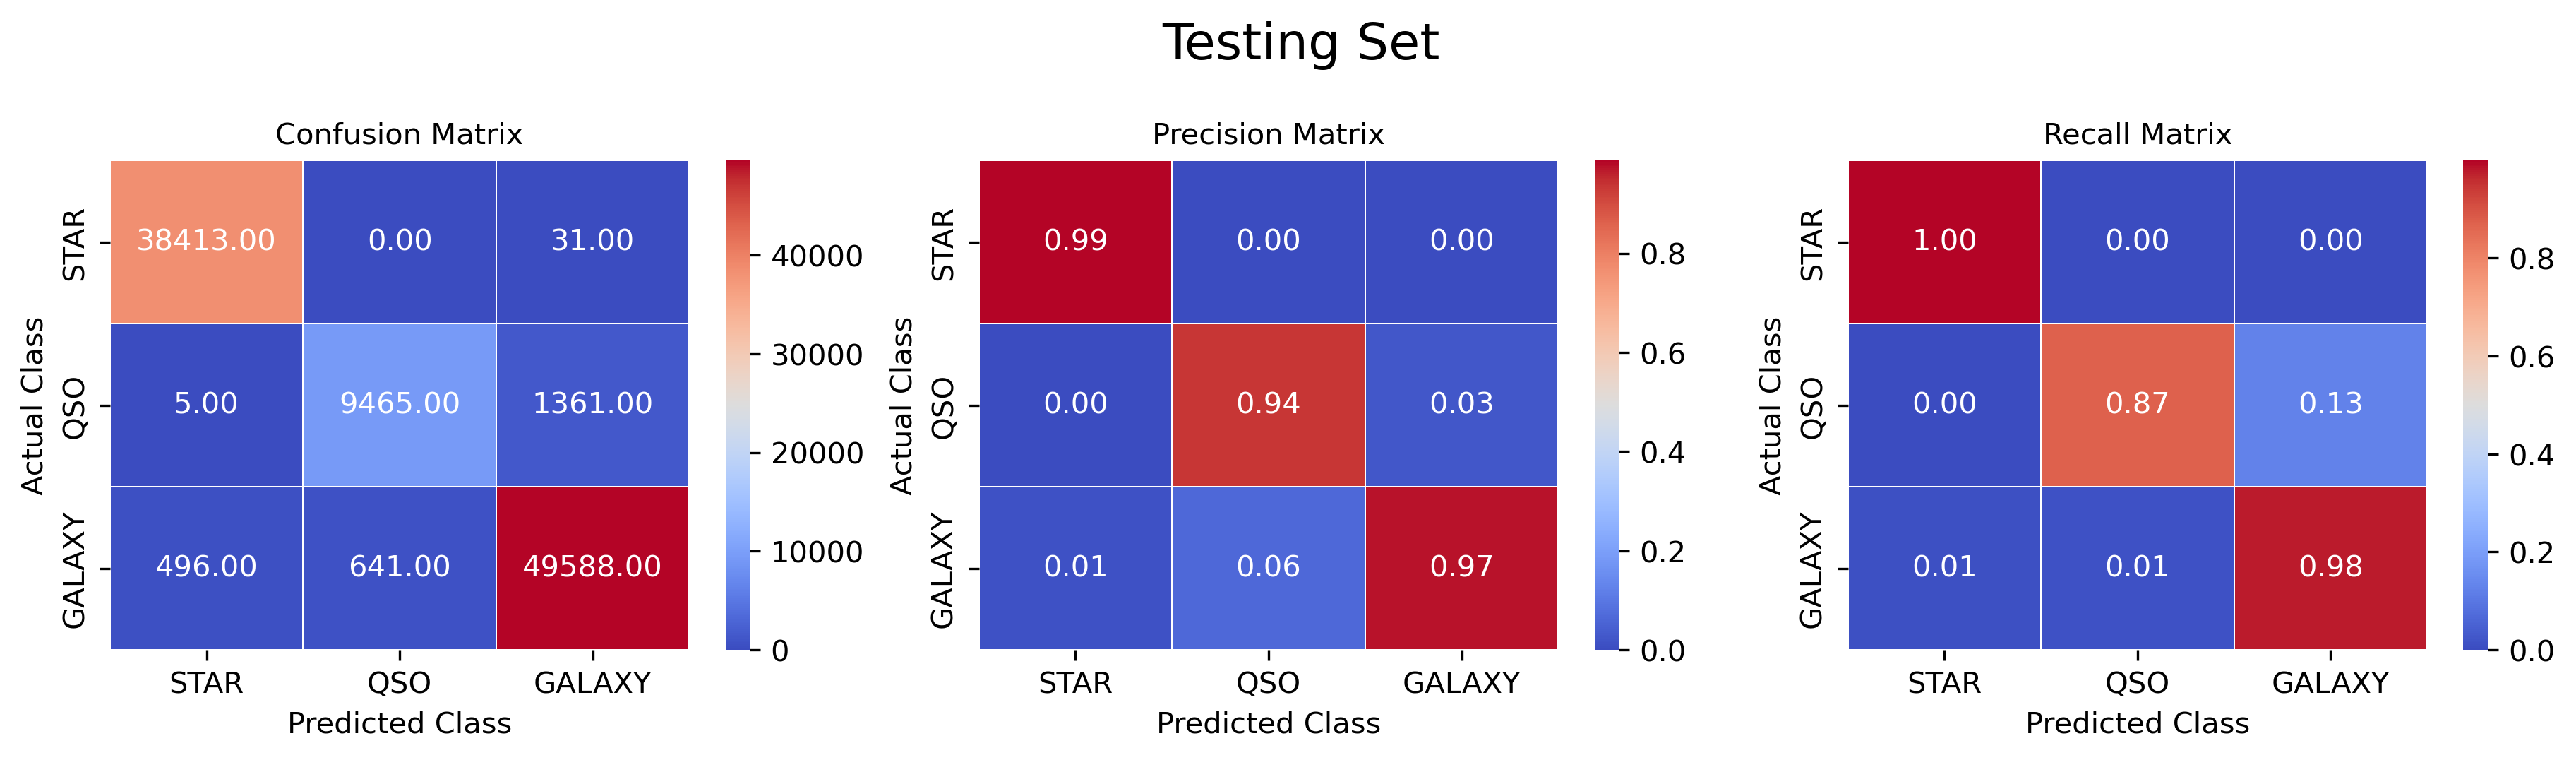
\includegraphics[width=\linewidth]{images/Baseline_RFC_Test.png}
        \caption{Testing Set Confusion Matrix, Precision and Recall}
        \label{fig:BaselineRFCTest}
    \end{subfigure}
    \begin{subfigure}{\textwidth}
        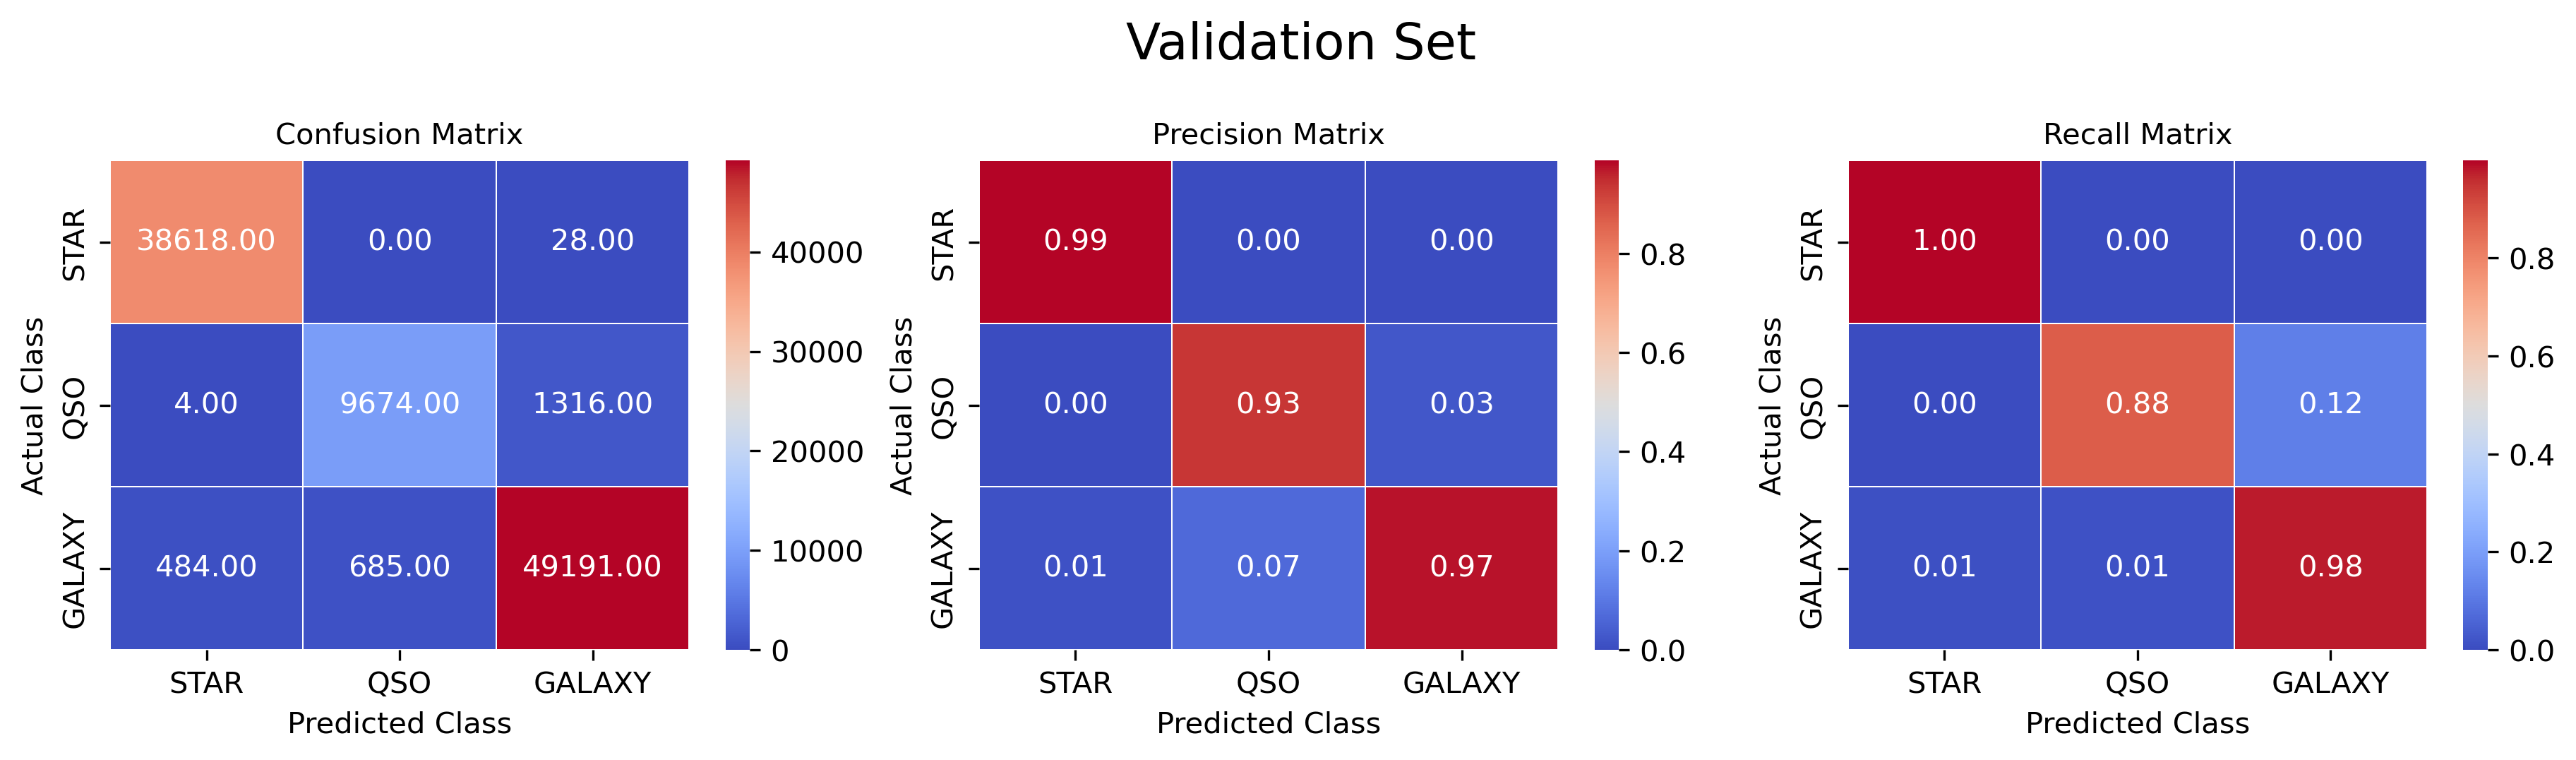
\includegraphics[width=\linewidth]{images/Baseline_RFC_Val.png}
        \caption{Validation Set Confusion Matrix, Precision and Recall}
        \label{fig:BaselineRFCVal}
    \end{subfigure}
    \caption{Baseline performance of Random Forest Classifier}
    \label{fig:BaselineRFC}
\end{figure}

After establishing the baseline for Random Forest Classifier we can apply genetic algorithm to tune the hyperparameters. From \autoref{sec:sectionrfc} we can choose hyperparameters and create a hyperparameter space. In the code block \autoref{lst:GARFC} this hyperparameter space is named \textit{param\_grid} and I chose 2 hyperparameters due to computational limits. The sklearn-genetic-opt library offers a useful module named sklearn\_genetic.space that serves as a valuable tool for defining the hyperparameter space in which the genetic algorithm operates. Researchers and practitioners can specify the types of values that hyperparameters can take on during the optimization procedure using this module. 

The module provides three distinct categories for defining the hyperparameter space:
\begin{itemize}
    \item \textbf{Continuous Space}: When dealing with continuous hyperparameters, the 'Continuous' space option comes into play. This functionality enables the generation of values that are continuous, either as integers or floating-point numbers. These values are generated from a specified distribution, allowing for a broad range of possibilities. When a hyperparameter such as learning rate requires a continuous range of values, this option becomes extremely valuable. With the ability to consider both integers and floats, a variety of scenarios can be accommodated.
    \item \textbf{Integer Space}: In scenarios where hyperparameters must exclusively be integers, the 'Integer' space option becomes valuable. This feature ensures that only whole numbers are taken into account when optimizing. The 'Integer' space is an ideal choice for hyperparameters that involve discrete steps, such as the number of layers in a neural network or the number of trees in a random forest.
    \item \textbf{Categorical Space}: Some hyperparameters present themselves in a categorical format, where the choices are expressed as strings or labels. The 'Categorical' space option addresses such scenarios by allowing the specification of a list of possible values. This approach is particularly useful when dealing with hyperparameters that correspond to specific configurations or options. For instance, a choice between different activation functions in a neural network or different kernel types in a support vector machine can be handled through the 'Categorical' space.
\end{itemize}
Using these distinct space options, the sklearn-genetic-opt library ensures that the genetic algorithm may be tailored to meet the needs of various hyperparameter types, enhancing its adaptability and effectiveness. As a result of defining the hyperparameter space in this manner, the optimization procedure is more efficient because the algorithm will be able to navigate the search space more effectively. Thus, it is more likely that optimal hyperparameter settings will be found, leading to enhanced performance of the model.

I have used StratifiedKFold for cross validation as our dataset has imbalanced classes, see \autoref{fig:classdistribution}. The function \textit{GASearchCV( )} from sklearn-genetic-opt library is used to apply genetic algorithm on the hyperparameter space. The functions take values which are genetic operators as mentioned in detail in \autoref{sec:geneticoperators}. These operators are selected based on official documentation and also keeping in mind the computational limitations, as larger values significantly slow down the search algorithm. The code used here takes about 20 minutes to train.

\begin{lstlisting}[language=Python, caption = {Applying Genetic algorithm on Random Forest Classifier}, label={lst:GARFC}]
param_grid = {'min_weight_fraction_leaf': Continuous(0.01, 0.5, distribution='log-uniform',
    random_state=random_seed),
    'n_estimators': Integer(100, 300,random_state=random_seed)}


cv = StratifiedKFold(n_splits=5, shuffle=True, random_state=random_seed)

rfc_genopt = GASearchCV(estimator=rfc,
                               cv=cv,
                               scoring='accuracy',
                               population_size=10,
                               generations=5,
                               tournament_size=3,
                               elitism=True,
                               crossover_probability=0.5,
                               mutation_probability=0.1,
                               param_grid=param_grid,
                               criteria='max',
                               algorithm='eaMuPlusLambda',
                               n_jobs=-1,
                               verbose=True,
                               keep_top_k=3)
# TAKES ABOUT 15-20 MINUTES TO RUN
rfc_genopt.fit(X_train,y_train)
\end{lstlisting}

Here's an explanation of each parameters used to instantiate the \textit{GASearchCV( )} object:
\begin{itemize}
    \item \textbf{estimator}: The machine learning model for which we want to optimize the hyperparameters. In this case it is `rfc' standing for random forest classifier.
    \item \textbf{cv}: Cross-validation strategy to be used for evaluating different hyperparameter configurations. In this case we have 5 fold cross validation using StratifiedKFold. Stratification takes case of class imbalance by maintaing the proportion of classes in K folds.
    \item \textbf{scoring}: The scoring metric used to evaluate the performance of different hyperparameter configurations. Common options are accuracy, precison and recall.
    \item \textbf{population\_size}: The number of individuals (candidate hyperparameter configurations) in each generation of the genetic algorithm.
    \item \textbf{generations}: The number of generations or iterations the genetic algorithm will run. Depending on available computing resources this number can be chosen by the practitioner. More the generations, better the search towards most optimum values.
    \item \textbf{tournament\_size}: The size of tournament selection process, where individuals compete to be selected for crossover and mutation.
    \item \textbf{elitism}: A boolean flag indicating whether elitism is enabled. Elitism preserves the best individuals from each generation to ensure they are passed to the next generation unchanged. This is analogous to the Darwin's rule of evolution - ``The strong one survives". In this case the ``strong" one is the one with maximum scoring metric.
    \item \textbf{crossover\_probability}: The probability of performing crossover(recombination) during genetic operations.
    \item \textbf{mutation\_probability}: The probability of performing mutation on individuals during genetic operation. Higher probability leads to wider search space exploration, but too high of a value will lead to the algorithm not finding the most optimum solution.
    \item \textbf{param\_grid}: The search space defined by the user with a range of values.
    \item \textbf{criteria}: The optimization criterion used to determine the best hyperparameter configuration. Options include 'max' (maximize the scoring metric) or 'min' (minimize the scoring metric).
    \item \textbf{algorithm}: The genetic algorithm variant to be used. Options include `eaSimple', `eaMuPlusLambda', `eaMuCommaLambda', etc. `eaMuCommaLambda' combines a mix of new individuals (lambda individuals) and the best individuals from the previous generation (mu individuals). However, in this case, the newly generated individuals completely replace the previous population. This can lead to more exploration of the solution space but may discard potentially good solutions from the previous generation.
    \item \textbf{n\_jobs}: The number of CPU cores used for parallel computation (-1 indicates using all available cores).
    \item \textbf{verbose}: If True, it prints progress updates during optimization.
    \item \textbf{keep\_top\_k}: The number of top individuals from each generation that are preserved for the next generation.

\end{itemize}

Here's the verbose printed while the Genetic algorithm is being used to search the hyperspace:
\begin{table}[H]
\centering
\caption{Genetic Algorithm verbose for Random Forest Classifier}
\label{tab:RFCverbose}
\begin{tabular}{|c|c|c|c|c|c|}
\hline
gen & nevals & fitness & fitness\_std & fitness\_max & fitness\_min \\
\hline
0   & 10     & 0.947509 & 0.0487177   & 0.97494     & 0.823433    \\
1   & 12     & 0.972395 & 0.00216501  & 0.97494     & 0.968843    \\
2   & 9      & 0.973929 & 0.00182915  & 0.97494     & 0.9692      \\
3   & 13     & 0.975158 & 0.000653    & 0.977117    & 0.97494     \\
4   & 13     & 0.975744 & 0.000683351 & 0.977117    & 0.97494     \\
5   & 14     & 0.976382 & 0.00048117  & 0.977117    & 0.976067    \\
\hline
\end{tabular}
\end{table}

\autoref{fig:GARFC} displays the performance of Random Forest model after genetic optimisation. 
\begin{figure}[H]
    \centering
    \begin{subfigure}{\textwidth}
        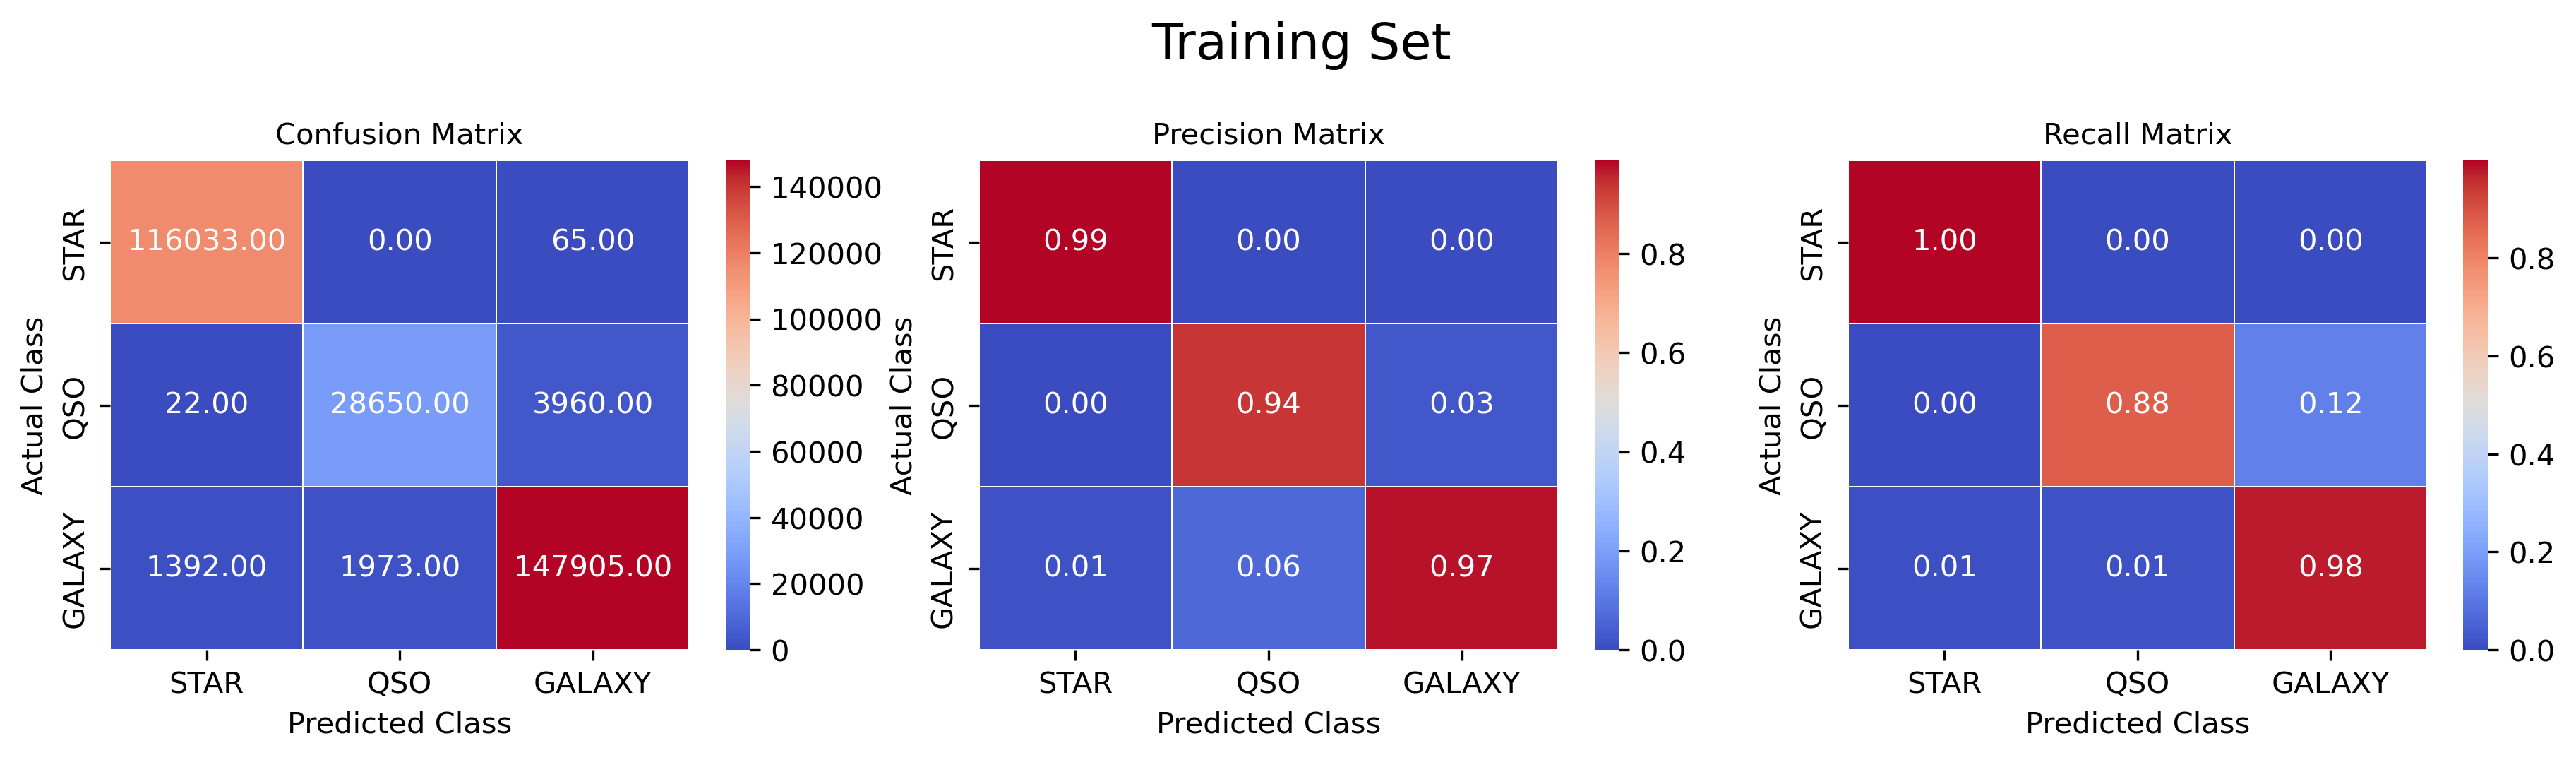
\includegraphics[width=\linewidth]{images/GA_RFC_Train.png}
        \caption{Training Set Confusion Matrix, Precision and Recall}
        \label{fig:GARFCTrain}
    \end{subfigure}
    \begin{subfigure}{\textwidth}
        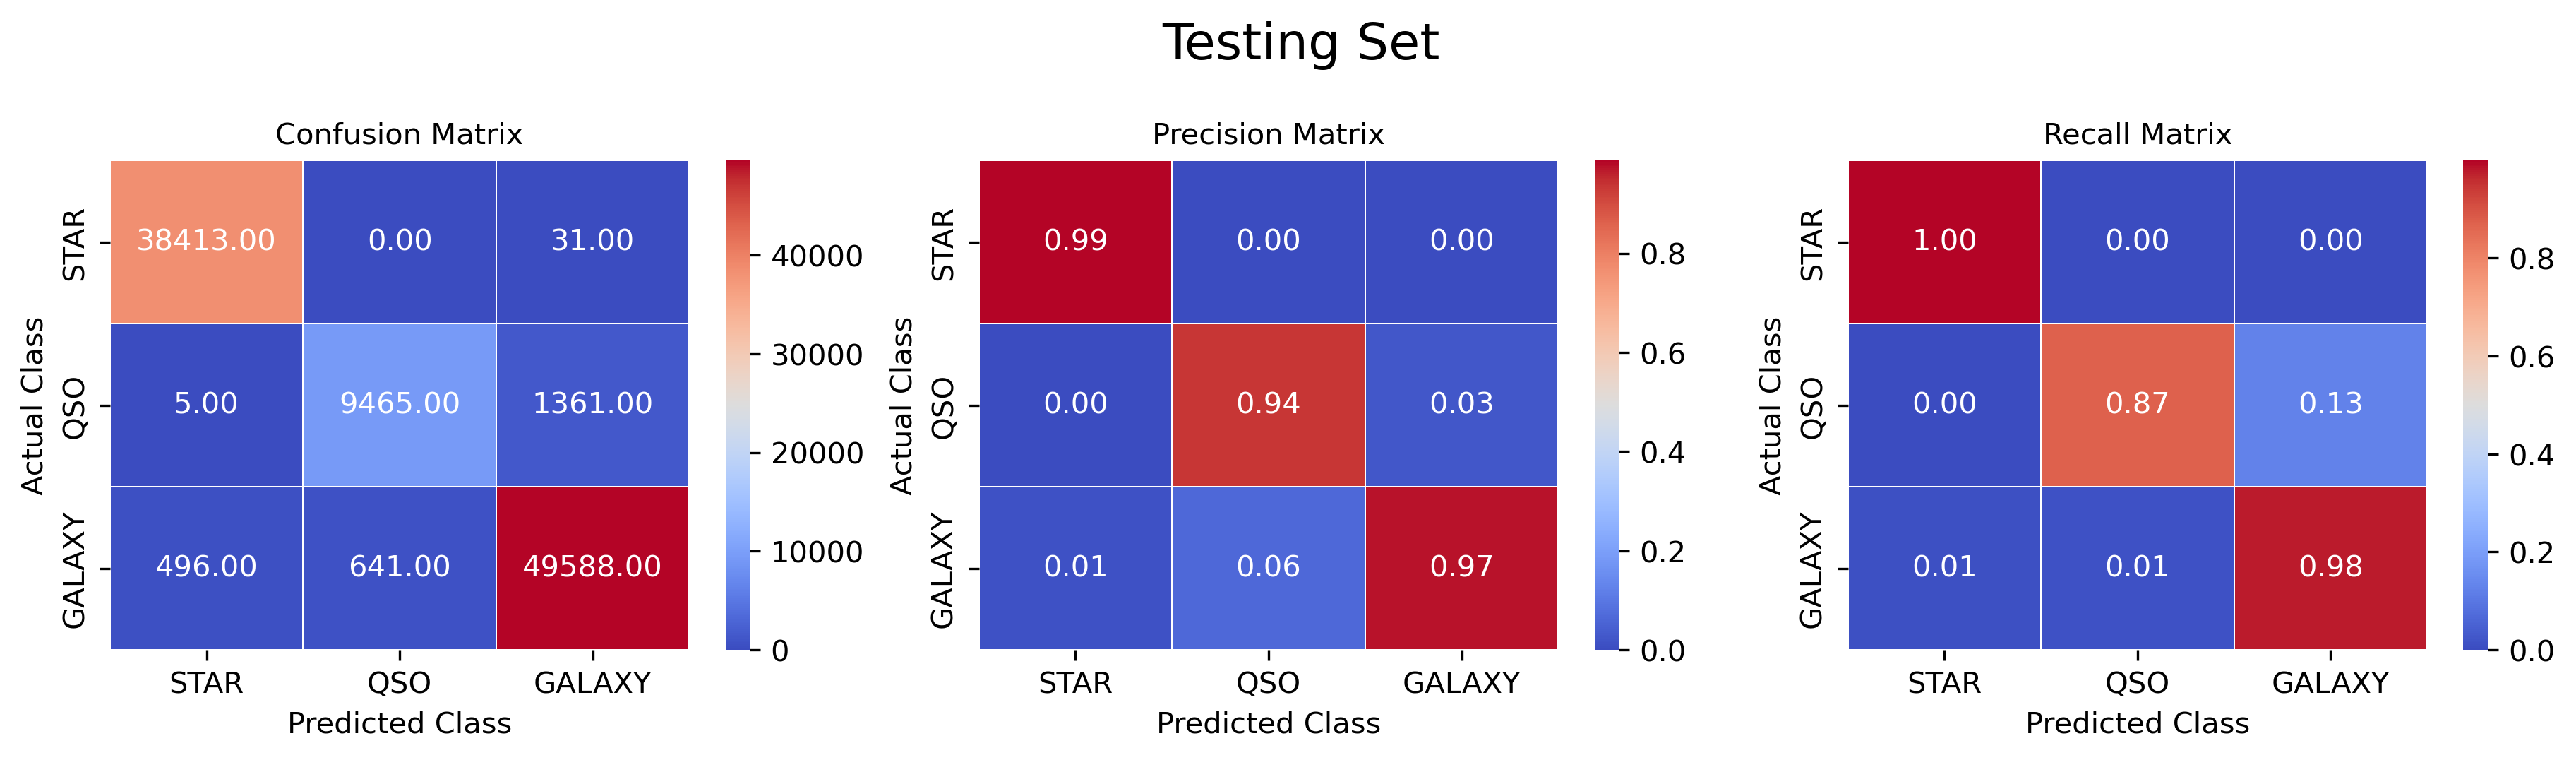
\includegraphics[width=\linewidth]{images/GA_RFC_Test.png}
        \caption{Testing Set Confusion Matrix, Precision and Recall}
        \label{fig:GARFCTest}
    \end{subfigure}
    \begin{subfigure}{\textwidth}
        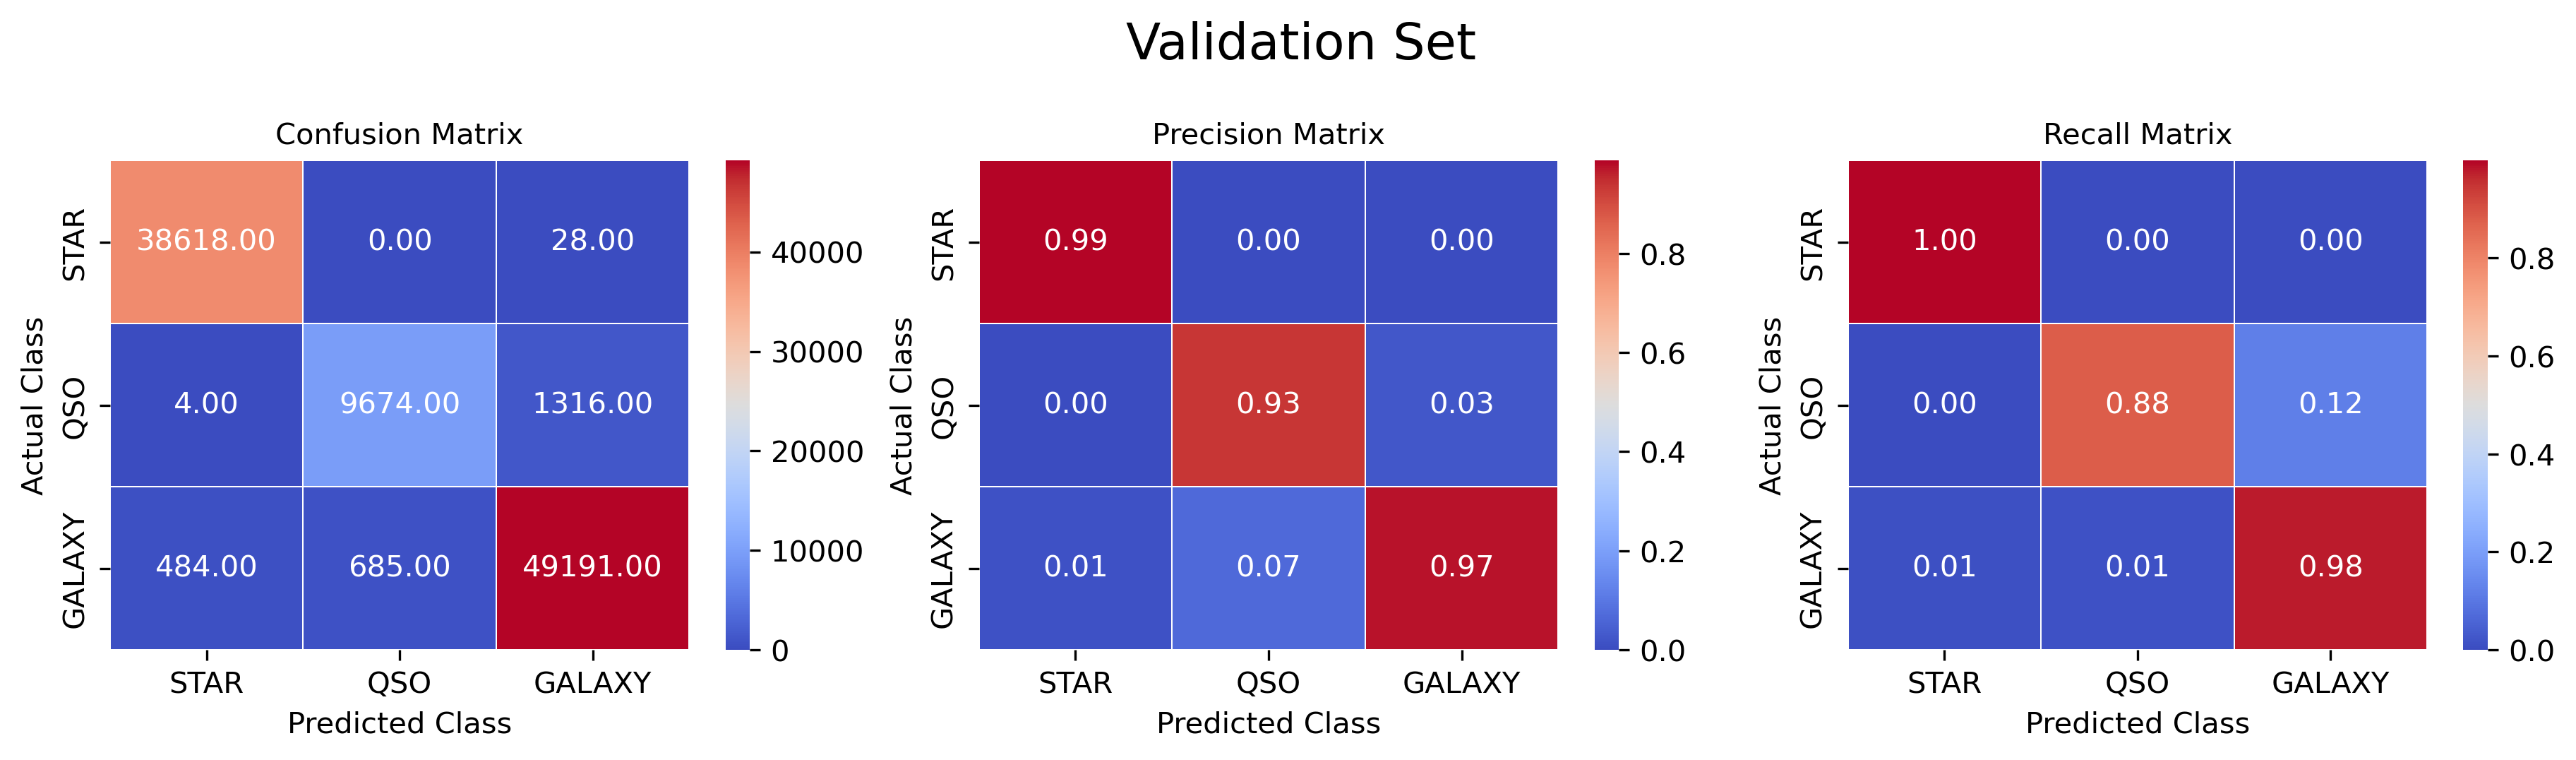
\includegraphics[width=\linewidth]{images/GA_RFC_Val.png}
        \caption{Validation Set Confusion Matrix, Precision and Recall}
        \label{fig:GARFCVal}
    \end{subfigure}
    \caption{Performance of Random Forest Classifier after Genetic optimisation}
    \label{fig:GARFC}
\end{figure}

\begin{table}[H]
\centering
\caption{Top 3 best Hyperparameters for Random Forest Classifier}
\begin{tabular}{|c|c|c|c|}
\hline
& 1 & 2 & 3 \\
\hline
min\_weight\_fraction\_leaf & 0.014455 & 0.014455 & 0.014455 \\
n\_estimators & 255.000000 & 257.000000 & 125.000000 \\
\hline
\end{tabular}
\end{table}
The default value of n\_estimators is 100 (this was recently changed to 100 from 10) and min\_weight\_fraction\_leaf is 0. But after using GA we are still getting very similar results if we round off to two decimal places. This mean either the change in values has no effect or our dataset is such that the model is able to learn or recognize the pattern very well. The later is more likely due to consistently high precision, recall and F1 scores both on testing and validation datasets.

\autoref{tab:RFCCompare} compares the metric values before (using default hyperparameters) and after (after genetic optimisation). We can see that there is hardly any change, the models are able to classify objects with very high precision and accuracy.

\begin{table}[H]
\centering
\caption{Before and After comparison of random forest classifier metrics of Validation set}
\label{tab:RFCCompare}
\begin{tabular}{|c|cc|cc|cc|cc|}
\hline
& \multicolumn{2}{c|}{Precision} & \multicolumn{2}{c|}{Recall} & \multicolumn{2}{c|}{F1-Score} & \multicolumn{2}{c|}{Accuracy}\\
\hline
& Before & After & Before & After & Before & After & Before & After\\
\hline
GALAXY & 0.97 & 0.97 & 0.98 & 0.97 & 0.98 & 0.98 & &\\
QSO    & 0.93 & 0.83 & 0.88 & 0.88 & 0.91 & 0.91 & 0.97 & 0.97\\
STAR   & 0.99 & 0.99 & 1.00 & 1.00 & 0.99 & 0.99 & & \\
\hline
\end{tabular}
\end{table}

\subsection{Gradient Boost Classifier}
We will follow the same framework as Random forest classifier, starting with establishing baseline performance of the model.

\begin{lstlisting}[language=Python]
    gbc = GradientBoostingClassifier(random_state=random_seed)
    # TAKES 5 MINUTES TO RUN
    gbc.fit(X_train, y_train)
\end{lstlisting}

After training the model with default hyperparameters, on both testing and validation datasets we get accuracy score of $\approx$ 0.98.

\begin{figure} 
    \centering
    \begin{subfigure}{\textwidth}
        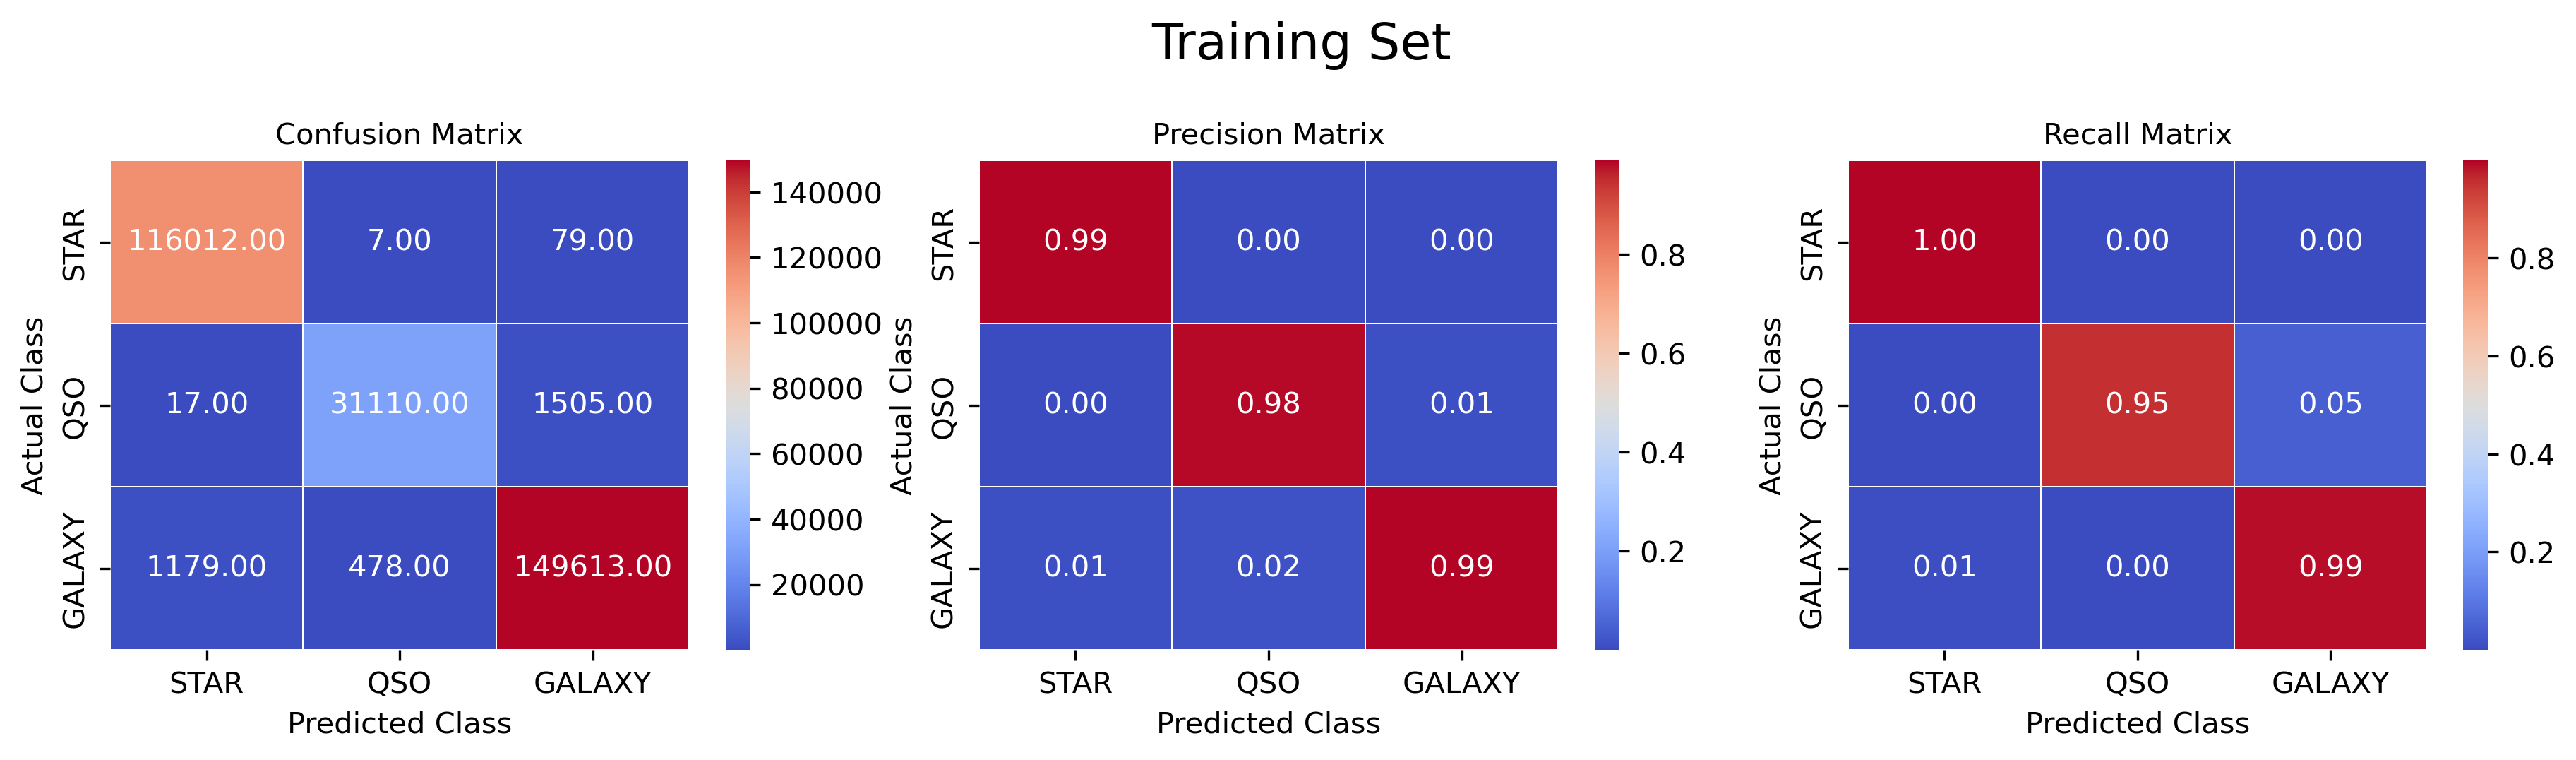
\includegraphics[width=\linewidth]{images/Baseline_GBC_Train.png}
        \caption{Training Set Confusion Matrix, Precision and Recall}
        \label{fig:BaselineGBCTrain}
    \end{subfigure}
    \begin{subfigure}{\textwidth}
        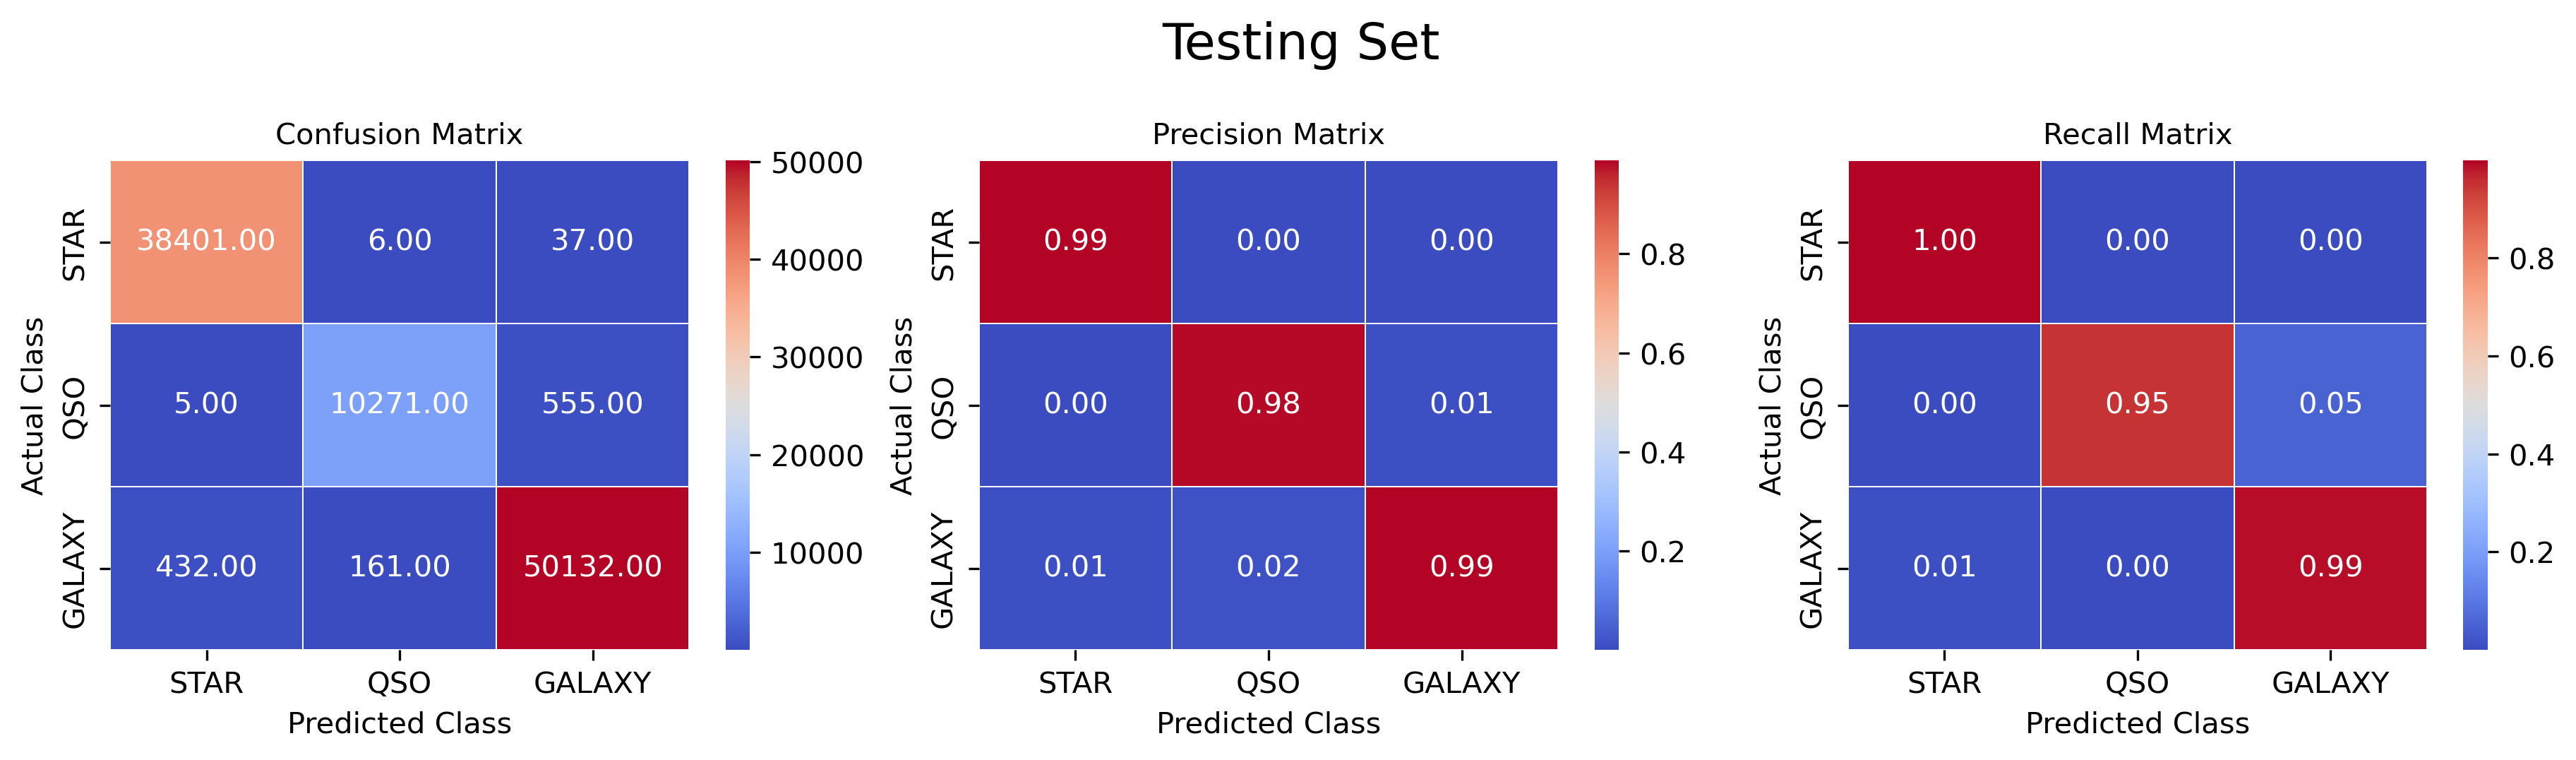
\includegraphics[width=\linewidth]{images/Baseline_GBC_Test.png}
        \caption{Testing Set Confusion Matrix, Precision and Recall}
        \label{fig:BaselineGBCTest}
    \end{subfigure}
    \begin{subfigure}{\textwidth}
        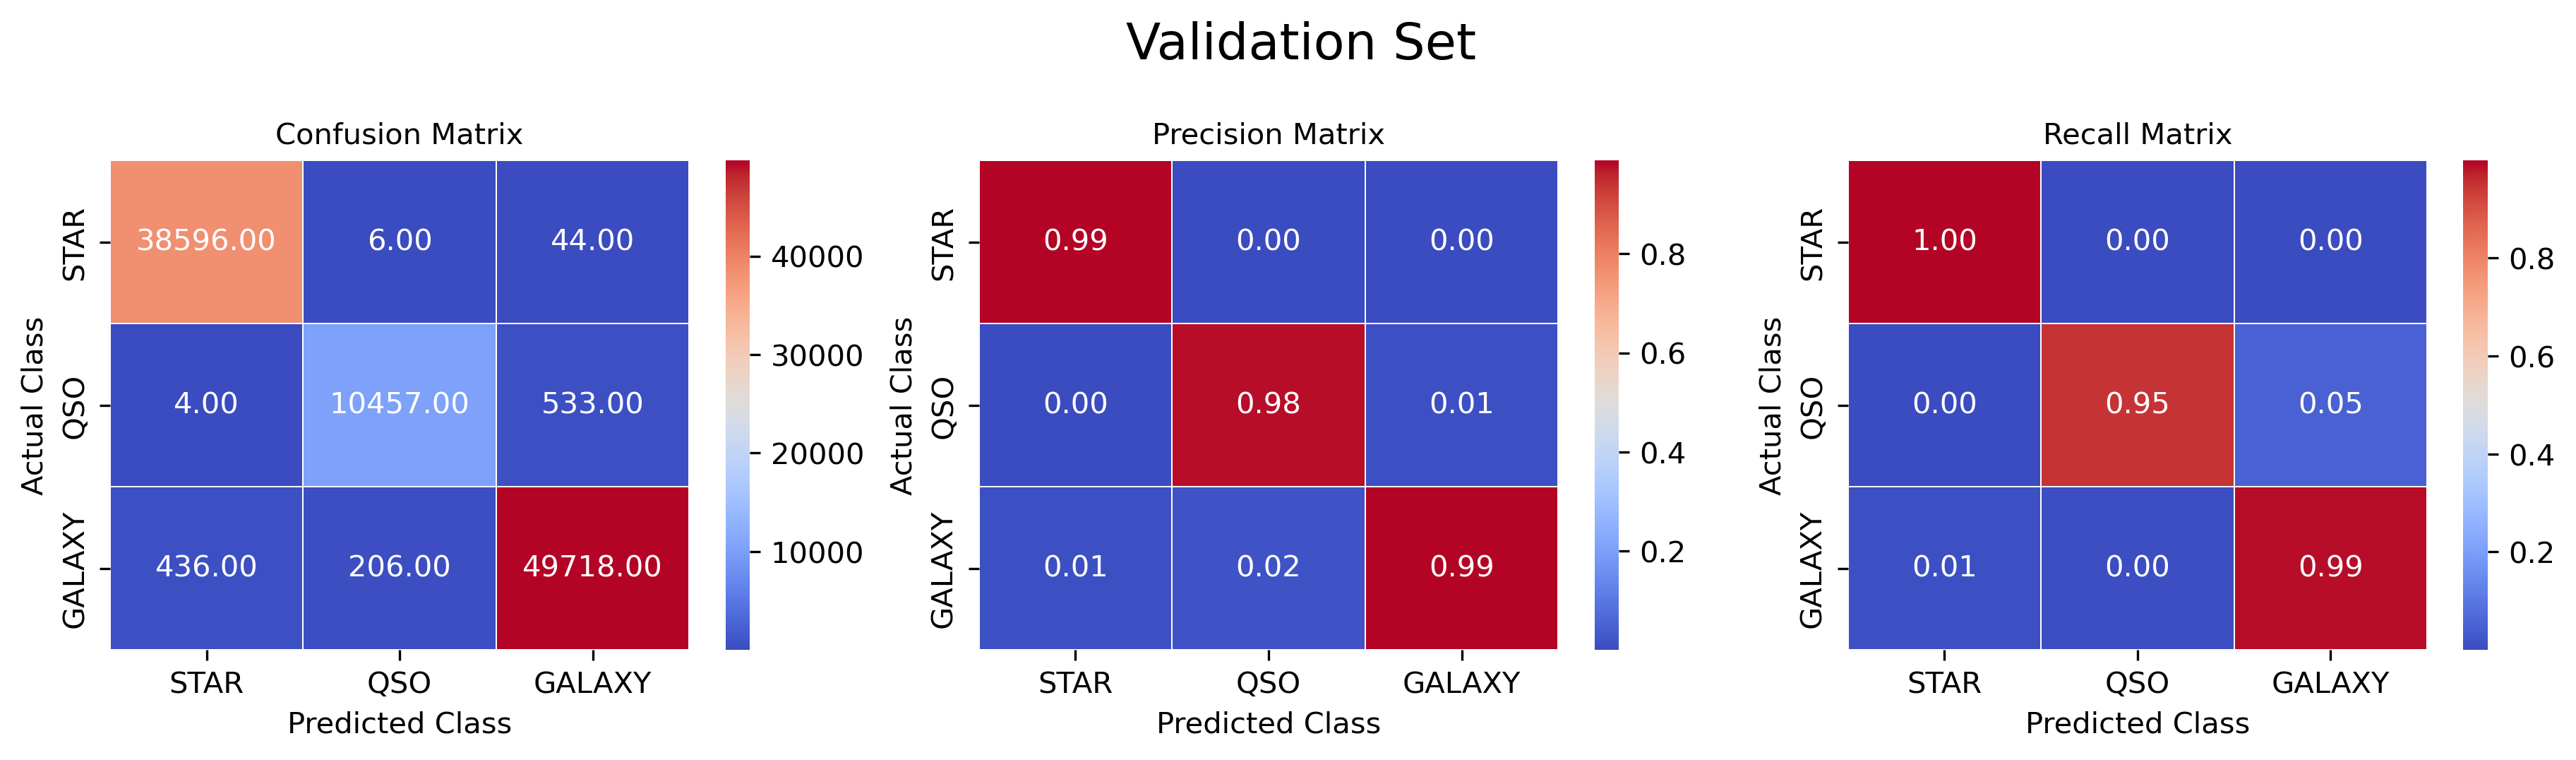
\includegraphics[width=\linewidth]{images/Baseline_GBC_Val.png}
        \caption{Validation Set Confusion Matrix, Precision and Recall}
        \label{fig:BaselineGBCVal}
    \end{subfigure}
    \caption{Baseline performance of Gradient Boosting Classifier}
    \label{fig:BaselineGBC}
\end{figure}

\autoref{fig:BaselineGBC} shows the confusion matrices with precision and recall scores for training, testing and validation scores. Even in this classifier we see good performance of model even on validation dataset.

From \autoref{sec:classifiergbc} we can choose hyperparameters and create a hyperparameter space. Work by \cite{Clarke2020} gives us an idea of important hyperparameters which influence the performance of machine learning models. Based on that and consider limited computational resources, I selected 2 hyperparameters (learning rate and n\_estimaters) to form my hyperparameter space. Even though learning rate is a float number, I have selected this hyperparameter as a categorical type consisting of 4 options, see \autoref{lst:GAGBC}

\begin{lstlisting}[language=Python, caption={Applying genetic algorithm to Gradient Boosting Classifer}, label={lst:GAGBC}]
gbc = GradientBoostingClassifier(random_state=random_seed)

param_grid = {
    'learning_rate': Categorical([0.0001, 0.001, 0.01, 0.1],random_state=random_seed),
    'n_estimators': Integer(50, 200, distribution='uniform',random_state=random_seed)
}

cv = StratifiedKFold(n_splits=5, shuffle=True, random_state=random_seed)

gbc_genopt = GASearchCV(estimator=gbc,
                               cv=cv,
                               scoring='accuracy',
                               population_size=5,
                               generations=5,
                               tournament_size=2,
                               elitism=True,
                               crossover_probability=0.5,
                               mutation_probability=0.1,
                               param_grid=param_grid,
                               criteria='max',
                               algorithm='eaMuPlusLambda',
                               n_jobs=-1,
                               verbose=True,
                               keep_top_k=3)
# TAKES ABOUT 240 MINUTES TO RUN
gbc_genopt.fit(X_train,y_train)
\end{lstlisting}

\begin{table}[H]
\centering
\caption{Genetic Algorithm verbose for Gradient Boosting Classifier}
\label{tab:GBCverbose}
\begin{tabular}{|c|c|c|c|c|c|}
\hline
gen & nevals & fitness & fitness\_std & fitness\_max & fitness\_min \\
\hline
0   & 5      & 0.850162 & 0.178689    & 0.98788     & 0.504233    \\
1   & 5      & 0.967104 & 0.0403195   & 0.98788     & 0.886483    \\
2   & 6      & 0.987343 & 0.000877902 & 0.98788     & 0.985597    \\
3   & 4      & 0.98777  & 0.000111355 & 0.98793     & 0.98768     \\
4   & 5      & 0.98776  & 9.79796e-05 & 0.98788     & 0.98768     \\
5   & 7      & 0.98784  & 8e-05       & 0.98788     & 0.98768     \\
\hline
\end{tabular}
\end{table}

From the verbose we can observe that the fitness (accuracy) approaches a similar value obtained from using default hyperparameters as generations increase.

\begin{figure}[H]
    \centering
    \begin{subfigure}{\textwidth}
        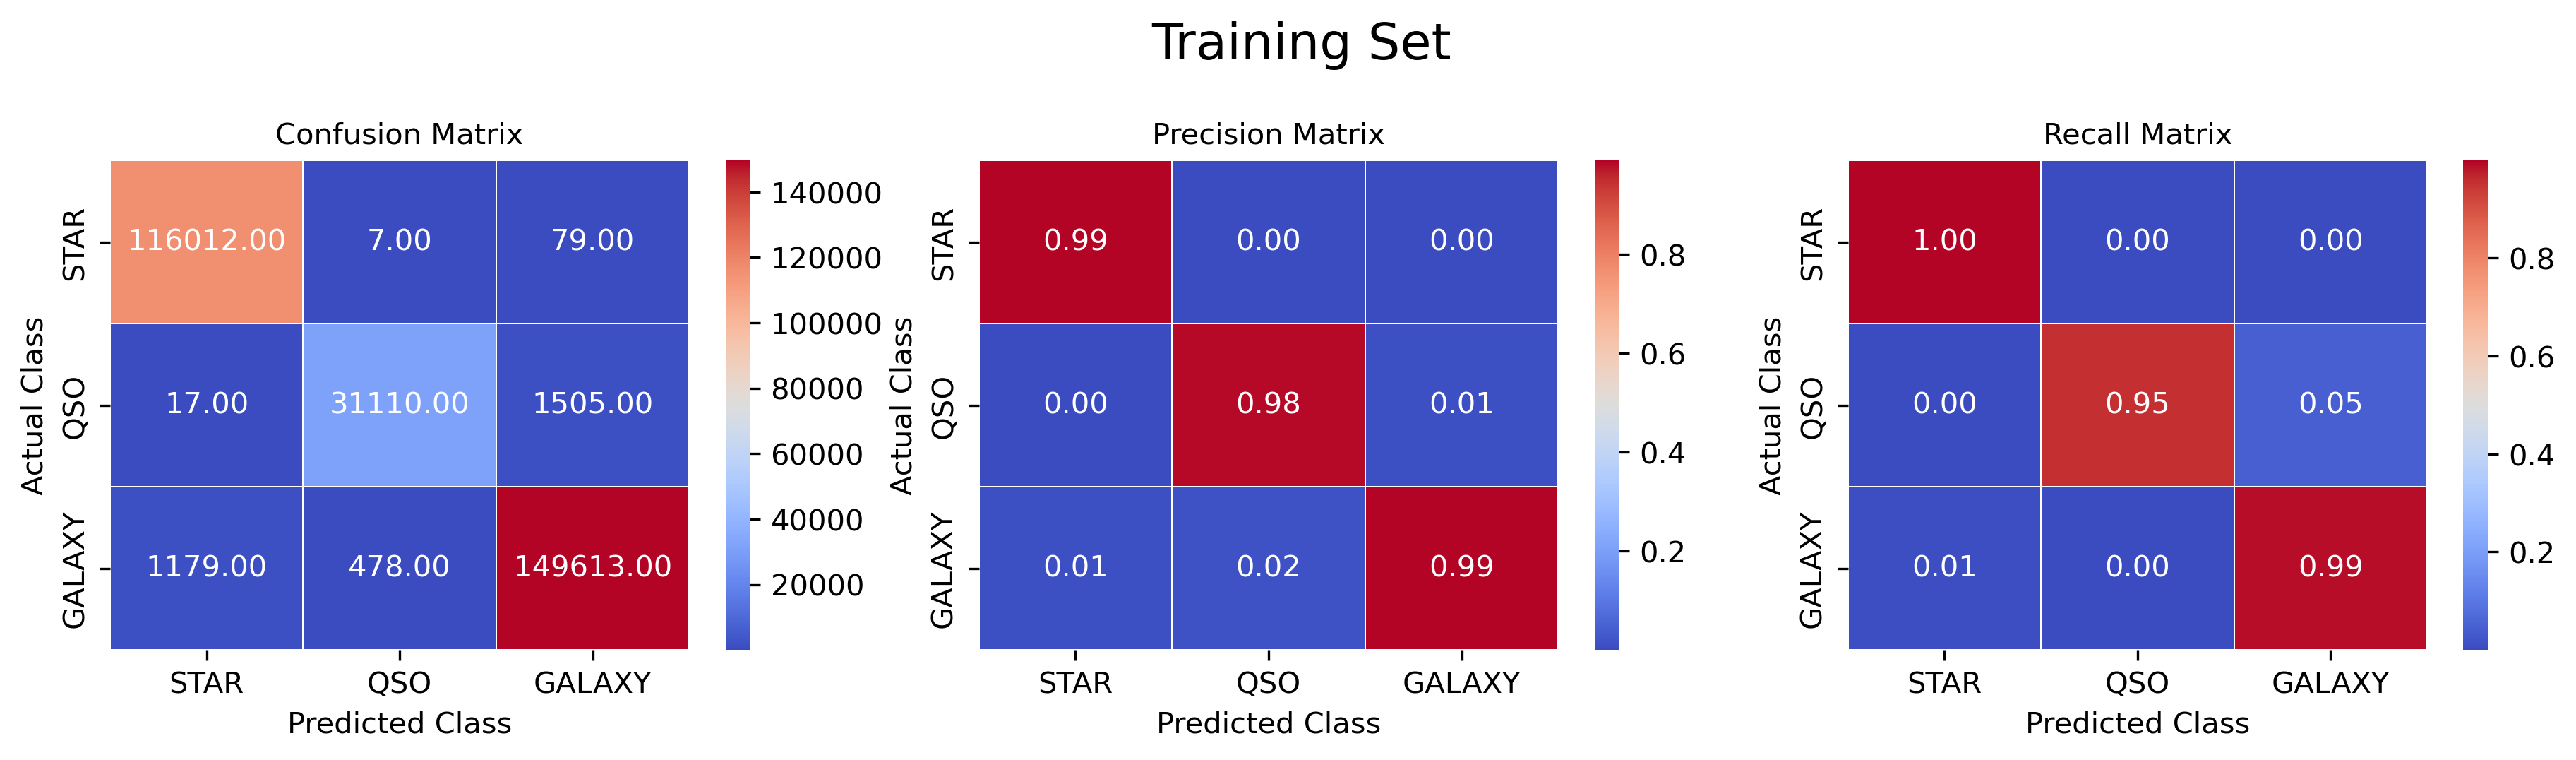
\includegraphics[width=\linewidth]{images/GA_GBC_Train.png}
        \caption{Training Set Confusion Matrix, Precision and Recall}
        \label{fig:GAGBCTrain}
    \end{subfigure}
    \begin{subfigure}{\textwidth}
        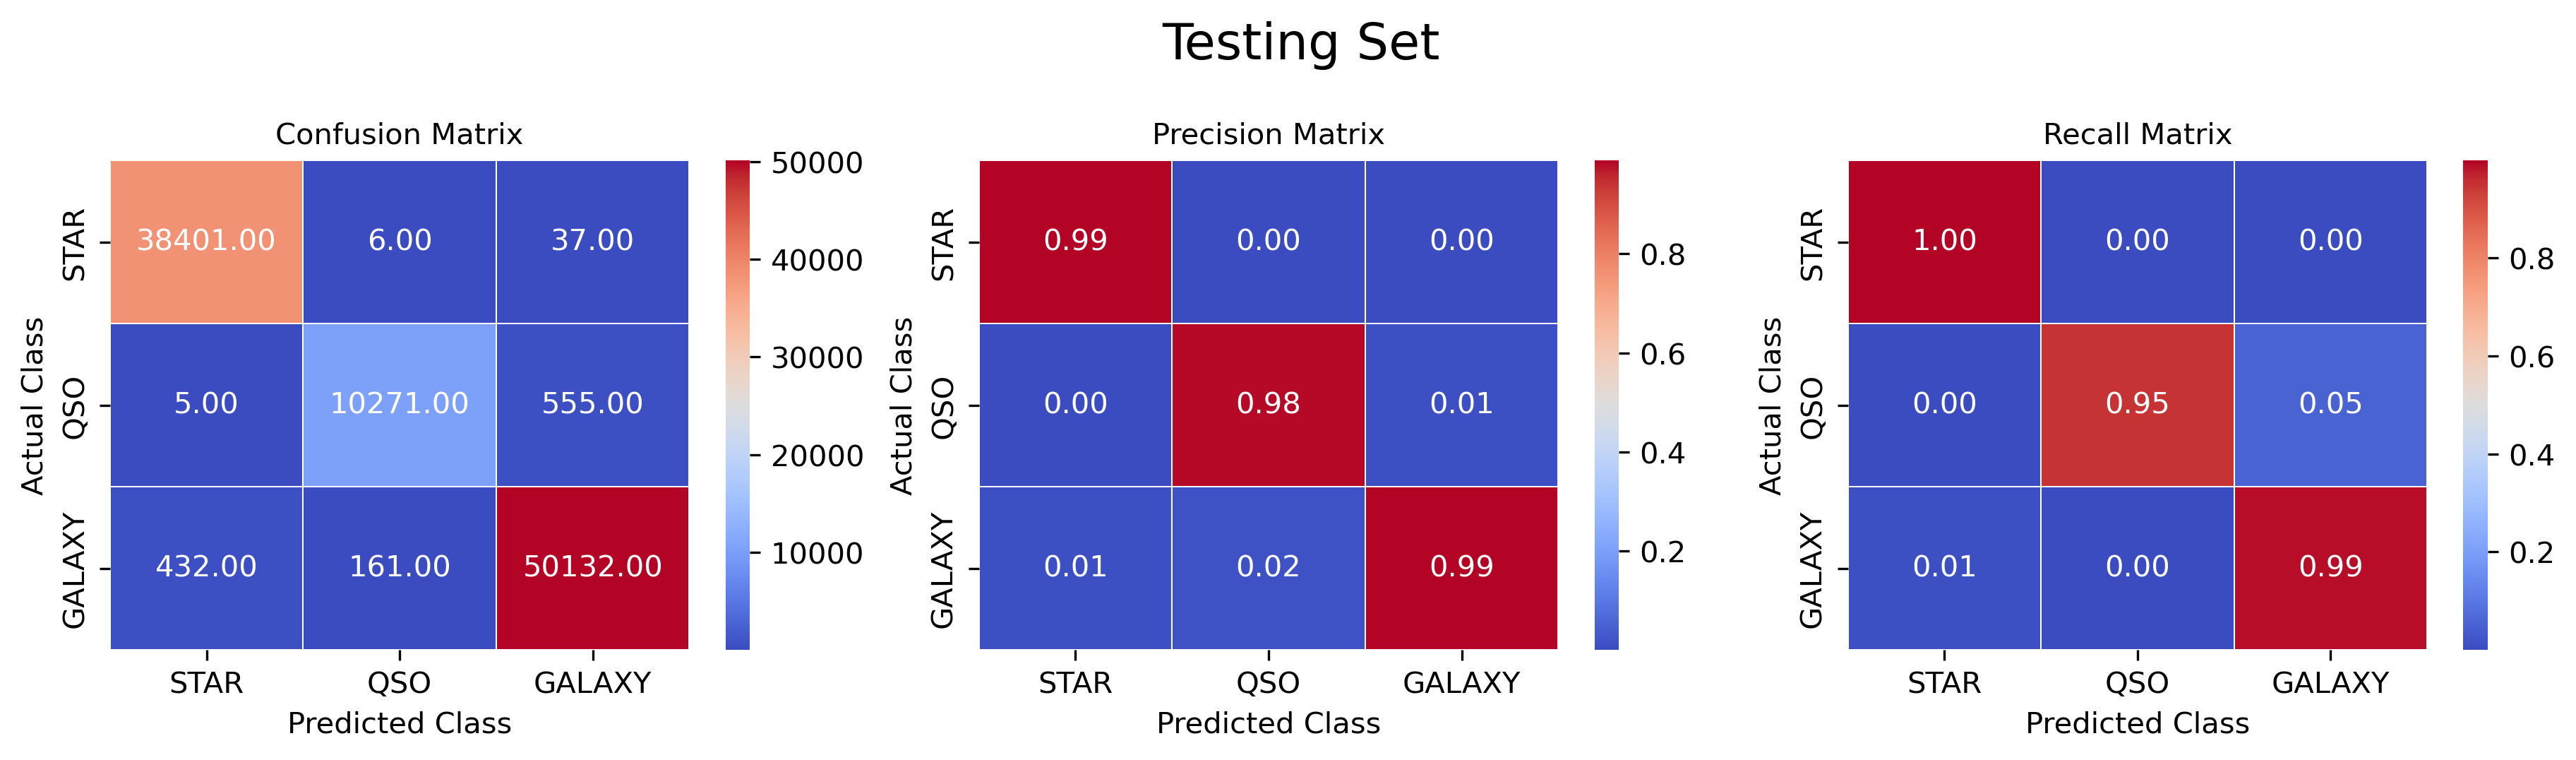
\includegraphics[width=\linewidth]{images/GA_GBC_Test.png}
        \caption{Testing Set Confusion Matrix, Precision and Recall}
        \label{fig:GAGBCTest}
    \end{subfigure}
    \begin{subfigure}{\textwidth}
        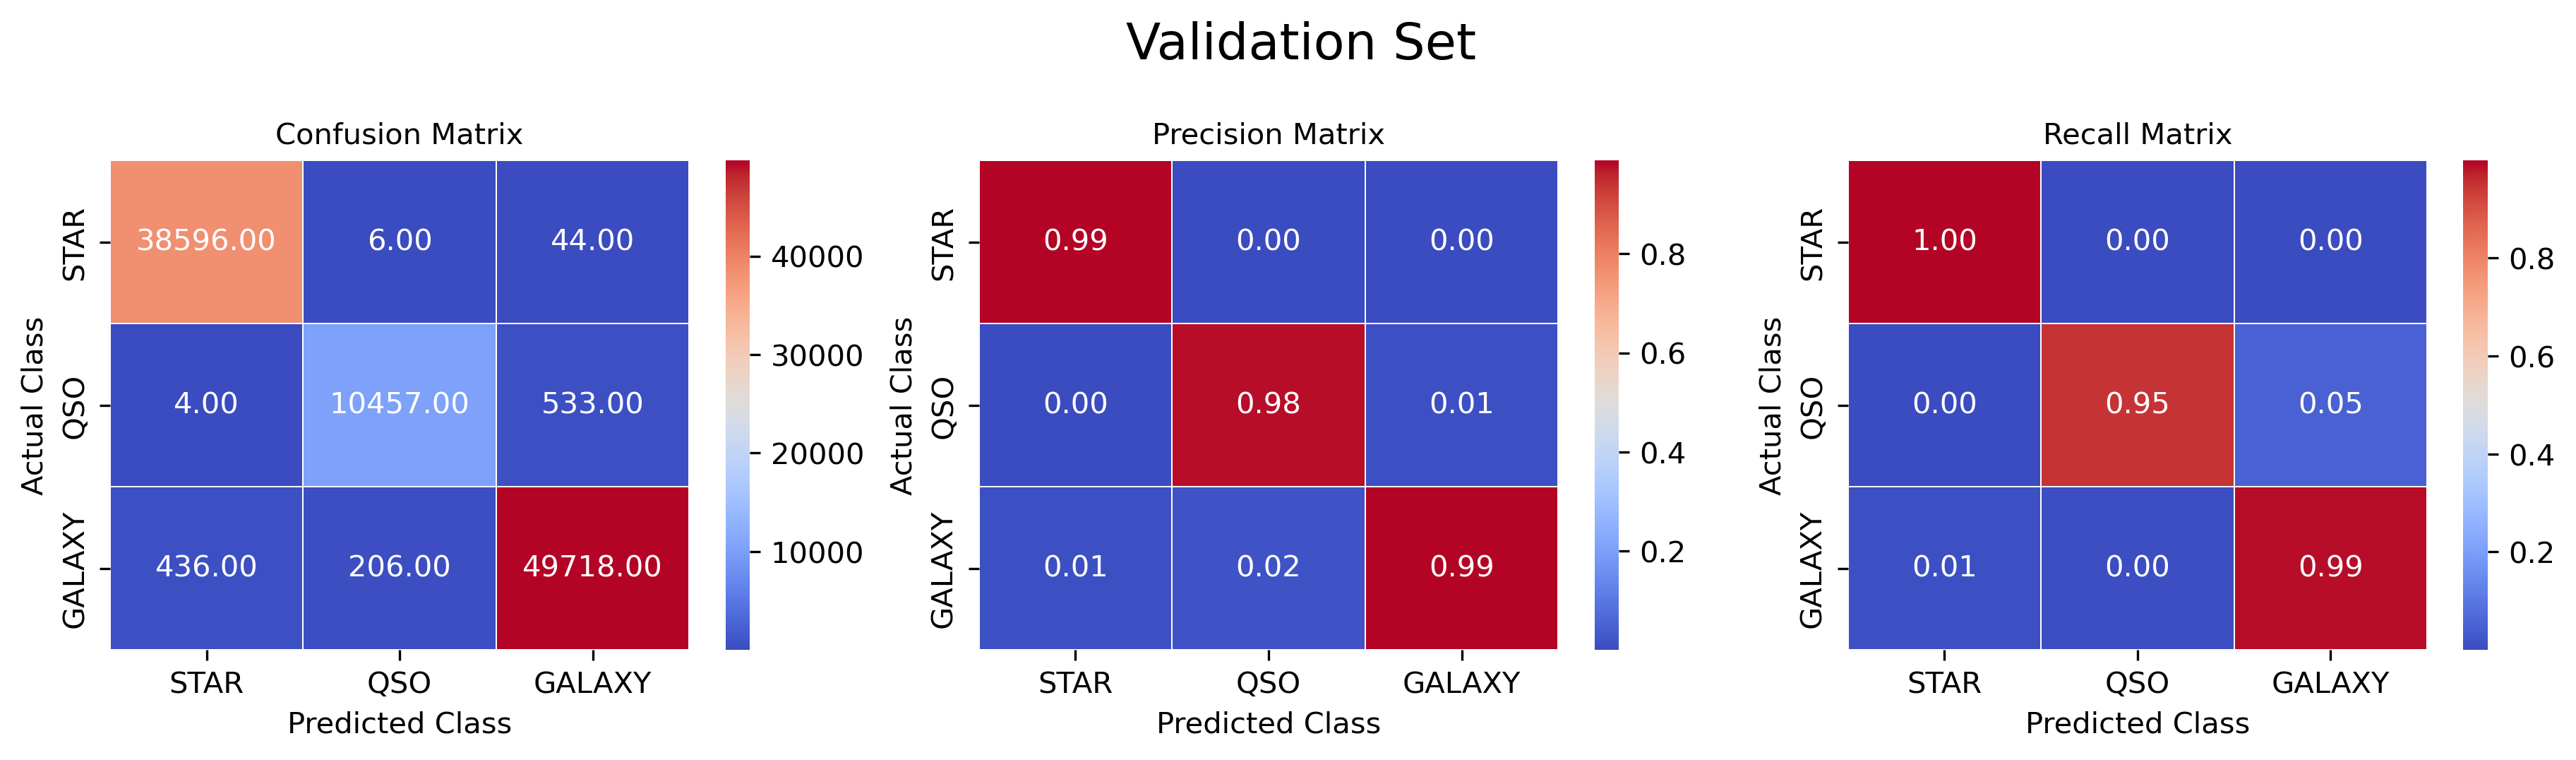
\includegraphics[width=\linewidth]{images/GA_GBC_Val.png}
        \caption{Validation Set Confusion Matrix, Precision and Recall}
        \label{fig:GAGBCVal}
    \end{subfigure}
    \caption{Performance of Gradient Boosting Classifier after Genetic optimisation}
    \label{fig:GAGBC}
\end{figure}

\begin{table}[H]
\centering
\caption{Top 3 best Hyperparameters for Gradient Boosting Classifier}
\begin{tabular}{|c|c|c|c|}
\hline
& 1 & 2 & 3 \\
\hline
learning\_rate & 0.1 & 0.1 & 0.1 \\
n\_estimators & 179.0 & 166.0 & 155.0 \\
\hline
\end{tabular}
\end{table}

The default value of n\_estimators is 100 and of learning\_rate is 0.1 which is consistent with what genetic optimisation yeilds. It is possible that the default hyperparameters are optimum for the dataset and it is able to learn the underlying patterns leading to such high metric scores in classification.

\begin{table}[H]
\centering
\caption{Before and After comparison of random forest classifier metrics of Validation set}
\label{tab:GBCCompare}
\begin{tabular}{|c|cc|cc|cc|cc|}
\hline
& \multicolumn{2}{c|}{Precision} & \multicolumn{2}{c|}{Recall} & \multicolumn{2}{c|}{F1-Score} & \multicolumn{2}{c|}{Accuracy}\\
\hline
& Before & After & Before & After & Before & After & Before & After\\
\hline
GALAXY & 0.99 & 0.99 & 0.99 & 0.99 & 0.99 & 0.99 & &\\
QSO    & 0.98 & 0.98 & 0.95 & 0.95 & 0.97 & 0.97 & 0.99 & 0.99\\
STAR   & 0.99 & 0.99 & 1.00 & 1.00 & 0.99 & 0.99 & & \\
\hline
\end{tabular}
\end{table}

Such high accuracy scores definitely raise suspicions of overfitting. To address this issue we considered Testing and validation set metrics and even they have very high values. In such a scenario it is possible that the data is such that the patterns are learned by the models resulting in highly accurate classification even on unseen dataset. In case of Gradient Boosting Classifier the precision, recall and F1 scores are exactly the same. The code with default hyperparameters takes about 2\% of the time it takes for genetic algorithm to search through the hyperparameter space. This indicates that the default values themselves are optimised values, especially for datasets with apparent patterns.

\subsection{Logistic Regression}
As a means of verifying the results I observed in the previous two models, I chose to use Logistic Regression. The logistic regression model uses regularisation and penalties to mitigate overfitting if it occurs in the previous two models. I was unsuccessful in my attempt to optimize hyperparameters of the Logistic Regression using genetic algorithms. Due to unknown reasons, sklean-genetic-opt was not working properly with logistic regression. There may be a compatibility issue between the penalties and the kind of solver used. The hyperparameter search space could not be explored due to the fact that not all solvers support all penalties. This means that problems of hyperparameter compatibility cannot be considered when exploring the hyperparameter search space.

I decided to proceed with default parameters as they have lead to high accuracy scores on previous models.

\begin{lstlisting}[language=Python, caption={Logistic Regression with default hyperparameters}, label={lst:Logreg}]
cv = StratifiedKFold(n_splits=5, shuffle=True, random_state=random_seed)
clf = LogisticRegressionCV(Cs=10, cv=cv, penalty='l2',solver='saga',n_jobs=-1,random_state=random_seed)
clf.fit(X=X_train, y=y_train)
\end{lstlisting}

\begin{table}[H]
\centering
\caption{Classification Report for Logistic regression on validation set}
\begin{tabular}{|c|c|c|c|}
\hline
& Precision & Recall & F1-Score \\
\hline
GALAXY & 0.99 & 0.98 & 0.98 \\
QSO & 0.98 & 0.94 & 0.96 \\
STAR & 0.97 & 1.00 & 0.99 \\
\hline
\end{tabular}
\end{table}

Upon reviewing the validation set classification report, it is evident that we still have high precision, recall, and F1 scores, suggesting that this is likely not the result of overfitting, since all models are giving high scores. This may be due to apparent patterns in the dataset, and such a situation may be unique to this type of dataset. 



\section{Limitations}


A prominent constraint that emerged during the study was the imposition of computational limitations. Genetic algorithms necessitate extensive parallel processing to efficiently explore the hyperparameter space. Despite this challenge, genetic algorithms are known for their capability to navigate the hyperparameter landscape and converge towards optimal values. This contrasted with alternative techniques such as random or grid search, which lack the assurance of identifying optimal solutions.

In addition, it is difficult to determine whether hyperparameters are compatible with each other since the search space is determined by the user. The ability to identify which hyperparameters do not work with others will be helpful, but it will also hinder the process of finding the most optimum value.